\documentclass[sn-mathphys,Numbered]{sn-jnl}

\usepackage{graphicx}
\usepackage{multirow}
\usepackage{amsmath,amssymb,amsfonts}
\usepackage{amsthm}
\usepackage{mathrsfs}
\usepackage{xcolor}
\usepackage{textcomp}
\usepackage{manyfoot}
\usepackage{booktabs}
\usepackage{tabularx}
\usepackage[title]{appendix}
\usepackage[version=4]{mhchem}

\graphicspath{{figures/}}

% Text-based ORCID iD link (the class's default \orcid needs Orcidlogo.eps, which is not bundled)
\gdef\orcid#1{\href{https://orcid.org/#1}{\textsuperscript{iD}}}

\begin{document}

\title[Thermodynamic and Kinetic Assessment of Ti Production]{Thermodynamic and Kinetic Assessment of Titanium Production via In-Situ Electrolysis and Bimetallic Complementary Reduction in \ce{MgCl2-CaCl2-NaCl-KCl} Molten Salt}

\author*{Yaming Hu\orcid{0009-0003-1406-0485}}\email{64687555@qq.com}

\affil*{Independent Researcher, Guiyang, Guizhou Province, China}

\abstract{This computational study proposes a novel titanium production process using a quaternary $\ce{MgCl2-CaCl2-NaCl-KCl}$ molten salt for in-situ electrolytic co-deposition of Mg and Ca for complementary reduction of $\ce{TiO2}$. Thermodynamic calculations ($\Delta G^{\circ} = -231.0$ to $-307.5$~kJ/mol at 600~$^{\circ}$C) show Ca deoxidation reaches 20~ppm versus 3908~ppm for Mg (194$\times$ difference), justifying the bimetallic strategy. Nernst analysis yields a $\ce{Ca^{2+}/Na+}$ co-deposition window of 120~mV (ideal), remaining positive (74.9--147.1~mV) under activity coefficient sensitivity ($\gamma_{\ce{CaCl2}} = 0.3$--1.0). The Mg--Ca liquid alloy ($\Delta G_{\mathrm{mix}} = -9.69$~kJ/mol) is thermodynamically stable. A shrinking-core model estimates complete reduction of 100~$\mu$m particles in 5.8~min ($D = 2.0\times10^{-9}$~m$^2$/s). Full-process energy balance, conditional on achieving $>$70\% current efficiency, indicates a net consumption of 11{,}192~kWh/ton-Ti (excluding impurity separation, which may add $\sim$2--4\%), with a second-law efficiency of $\sim$40.7\% based on the $\ce{TiO2 -> Ti + O2}$ reversible work of 4{,}550~kWh/ton-Ti. A Monte Carlo analysis with a broad current-efficiency distribution ($\eta_I \sim \mathrm{Tri}(0.50, 0.75, 0.88)$) yields $P(W < 14{,}000) = 85.8\%$, highlighting significant sensitivity to this unvalidated parameter. All quantitative results are theoretical predictions based on ideal solution assumptions and literature parameters. The process viability hinges critically on two unvalidated prerequisites: (i) sufficient MgO/CaO solubility ($\gtrsim$0.5~wt\%) at 600~$^{\circ}$C in the quaternary melt to close the salt loop, and (ii) sustained current efficiency $>$0.70 via a durable oxygen-evolving inert anode. Experimental validation of these bounds is mandatory before any pilot-scale assessment.}

\keywords{Titanium production; Quaternary chloride molten salt; Bimetallic complementary reduction; Electrochemical co-deposition; Thermodynamic modeling; Shrinking core kinetics}

\maketitle

\section{Introduction}

Titanium is a strategic material for aerospace, marine engineering, and energy applications owing to its low density, high specific strength, and exceptional corrosion resistance. However, widespread civilian use remains limited by high production costs. The Kroll process, the dominant industrial route, requires multiple batch operations---chlorination, magnesiothermic reduction, and vacuum distillation---resulting in high energy consumption, severe pollution, and intermittent production \cite{kroll1937,ji2026}.

The core challenge in titanium metallurgy lies in the extremely high Ti--O bond energy, making efficient deoxidation difficult, while titanium's chemical reactivity at elevated temperatures leads to contamination by N, H, and C. Molten salt electrolysis has emerged as a promising alternative. The FFC Cambridge process \cite{fray2000} directly reduces $\ce{TiO2}$ cathodically in $\ce{CaCl2}$ melt, but suffers from low current efficiency and difficult product separation. The USTB process \cite{jiao2023} uses electrochemical dissolution-deposition of titanium anodes but faces anode durability issues. The OS process \cite{ono2002} performs calciothermic reduction of $\ce{TiO2}$ in $\ce{CaCl2}$ melt with electrolytic regeneration of Ca, sharing the ``electrolytic regeneration of reductant'' concept with the present work. The SOM process \cite{pal2001} employs a solid oxide membrane to separate the anode from the melt, achieving higher current efficiency. Okabe et al.\ \cite{okabe1997} developed the electronically mediated reaction (EMR) approach for titanium production. Several review articles have summarized recent progress \cite{zhang2024,ji2026}.

Recent studies have explored $\ce{MgCl2}$-based salt systems for titanium production. Taninouchi et al. \cite{taninouchi2016} demonstrated electrochemical deoxidation of titanium in molten $\ce{MgCl2}$. Lee et al. \cite{lee2025} investigated $\ce{CaMg2}$ as a reductant for $\ce{TiO2}$. Pang et al. \cite{pang2024} achieved ultralow-oxygen titanium by direct reduction. Zhu et al. \cite{xu2025} produced low-oxygen titanium powder by molten salt electrolysis--magnesiothermic reduction. However, these approaches employ single-metal reduction, binary/ternary salt systems, and batch operation requiring preformed cathodes, differing in salt composition, reduction mechanism, and operational design from the process proposed here.

This paper proposes a quaternary $\ce{MgCl2-CaCl2-NaCl-KCl}$ molten salt system enabling in-situ electrolytic co-deposition of Mg and Ca for complementary reduction of $\ce{TiO2}$. The key innovation is an electrochemical-thermochemical coupling: Mg provides fast reduction kinetics while Ca delivers deep deoxidation. The by-product oxides ($\ce{MgO}$, $\ce{CaO}$) dissolve in the $\ce{CaCl2}$-containing melt and are electrolytically regenerated, establishing a closed-loop cycle. This work presents a comprehensive thermodynamic, electrochemical, and kinetic assessment using established databases \cite{barin1995,waldner1999} and literature parameters, providing a quantitative theoretical framework. The specific novelties of this study are:

\begin{itemize}
\item To the authors' knowledge, the first proposal of in-situ electrolytic co-deposition of Mg and Ca in a quaternary $\ce{MgCl2-CaCl2-NaCl-KCl}$ molten salt for titanium production, combining Mg's kinetic advantage with Ca's thermodynamic deoxidation depth in a single closed-loop process. While bimetallic Mg--Ca reductants (e.g., $\ce{CaMg2}$ \cite{lee2025}), $\ce{MgCl2}$-based deoxidation \cite{taninouchi2016}, and electrolytic Ca regeneration in the OS process \cite{ono2002} have been studied, the in-situ electrolytic co-deposition of both Mg and Ca in a quaternary system is novel.
\item The CALPHAD-derived Redlich--Kister parameters of the Mg--Ca system reported by Zhang et al.\ \cite{zhang2008mgce} are introduced to characterize alloy mixing behavior. Additionally, the robustness of the $\ce{Ca^{2+}/Na+}$ co-deposition window is evaluated by combining Nernst-equation calculation, activity-coefficient sensitivity analysis, and overpotential qualitative analysis.
\item Kinetic prediction via the shrinking core model with multi-parameter sensitivity analysis ($D = 1$--$3\times10^{-9}$~m$^2$/s, $\varepsilon = 0.1$--0.5, $\tau = 1.5$--5.0), providing reduction time estimates for process design.
\item Full-process energy and exergy analysis (11{,}192~kWh/ton-Ti net consumption, \emph{theoretical prediction conditional on $\eta_I > 0.70$}; process energy efficiency 54.6\%, electrolysis energy fraction 93.9\%) with preliminary comparison to both Kroll and FFC routes, acknowledging boundary differences.
\end{itemize}

This work is a conceptual feasibility study conducted independently: all thermodynamic, electrochemical, and kinetic calculations, data processing, and uncertainty analyses were performed computationally by the author from published data and open-source tooling, without access to institutional laboratory facilities. The results are therefore intended as a quantitative design basis for subsequent experimental validation.

\section*{Nomenclature}

\begin{tabular}{ll}
\multicolumn{2}{l}{\textit{Thermodynamic quantities}} \\
$\Delta G^{\circ}$ & Standard Gibbs free energy change (kJ/mol) \\
$\Delta H^{\circ}$ & Standard enthalpy change (kJ/mol) \\
$\Delta S^{\circ}$ & Standard entropy change (J/(mol$\cdot$K)) \\
$\Delta G_{\mathrm{mix}}$ & Mixing Gibbs free energy of Mg--Ca alloy (kJ/mol) \\
$\Delta G_{\mathrm{deox}}$ & Deoxidation free energy, per 1~mol O basis (kJ/mol) \\
$\Delta G_{\mathrm{diss}}$ & Dissolution free energy of O in $\alpha$-Ti (J/mol) \\
$\Delta H_{\mathrm{fus}}$ & Enthalpy of fusion (kJ/mol) \\
$C_p$ & Heat capacity (J/(mol$\cdot$K)) \\
$K$ & Equilibrium constant \\
\multicolumn{2}{l}{\textit{Electrochemical quantities}} \\
$E^{\circ}_{\mathrm{red}}$ & Standard reduction potential (V) \\
$E_{\mathrm{red}}$ & Reduction potential (V) \\
$E_d$ & Decomposition voltage (V) \\
$\Delta E$ & Co-deposition window (mV) \\
$n$ & Number of electrons transferred \\
$a$ & Activity \\
$\gamma$ & Activity coefficient \\
$p_{\ce{O2}}$ & Oxygen partial pressure (atm) \\
\multicolumn{2}{l}{\textit{Physical constants}} \\
$R$ & Universal gas constant, 8.314 J/(mol$\cdot$K) \\
$F$ & Faraday constant, 96{,}485 C/mol \\
\multicolumn{2}{l}{\textit{Process variables}} \\
$T$ & Temperature (K or $^{\circ}$C as indicated) \\
$T_m$ & Melting temperature (K) \\
$x_i$ & Mole fraction of component $i$ \\
$D$ & Diffusion coefficient (m$^2$/s) \\
$D_{\mathrm{eff}}$ & Effective diffusion coefficient, $D\varepsilon/\tau$ (m$^2$/s) \\
$\varepsilon$ & Porosity \\
$\tau$ & Tortuosity \\
$c_{\mathrm{O}}$ & Oxygen concentration in TiO$_2$ (mol/m$^3$) \\
$c_{\mathrm{red}}$ & Reductant concentration (mol/m$^3$) \\
$M_{\mathrm{avg}}$ & Effective molar mass of the reductant-bearing melt ($\approx$85 g/mol) \\
$\eta_I$ & Current efficiency \\
$V_{\mathrm{cell}}$ & Cell voltage (V) \\
$\Omega$ & Interaction parameter (kJ/mol) \\
$L_0$ & Zeroth-order Redlich--Kister parameter (J/mol) \\
$L_1$ & First-order Redlich--Kister parameter (J/mol, neglected in this work) \\
$w_{[\mathrm{O}]}$ & Equilibrium oxygen content (wt\%) \\
$p_{\mathrm{O}^{2-}}$ & Negative logarithm of oxide ion activity, $-\log_{10}(a_{\mathrm{O}^{2-}})$ \\
$n_{\mathrm{Ti}}$ & Moles of Ti per metric ton ($\mathrm{mol/ton}$) \\
\end{tabular}

\section{Process Description}

The proposed process is designed over a 580--650~$^{\circ}$C operating range, with 600~$^{\circ}$C taken as the nominal \emph{design-basis} temperature at which all thermodynamic and kinetic figures herein are reported. Because of the liquidus uncertainty (Limitations~(4)), a pilot-scale operating floor of $\geq$620~$^{\circ}$C is recommended; the shift from 600 to 620~$^{\circ}$C changes the energy and co-deposition-window figures by only a few percent and does not alter the qualitative conclusions. The melt is a quaternary $\ce{MgCl2-CaCl2-NaCl-KCl}$ mixture. $\ce{MgCl2}$ serves as the primary salt and magnesium source; $\ce{CaCl2}$ enhances oxide solubility and lowers the melting point; NaCl and KCl act as fluxes to improve ionic conductivity and reduce viscosity \cite{sato1999}. The operational cycle consists of: (i) electrolytic co-deposition of Mg and Ca at the cathode; (ii) reduction of $\ce{TiO2}$ powder by the co-deposited metals; (iii) dissolution of $\ce{MgO}$ and $\ce{CaO}$ in the melt; and (iv) electrolytic regeneration of $\ce{Mg^{2+}}$ and $\ce{Ca^{2+}}$ with oxygen evolution at the anode. The net reaction is $\ce{TiO2 -> Ti + O2}$, driven by electrical energy, with Mg and Ca acting as cyclic mediators.

\section{Thermodynamic Framework}

\subsection{Data Sources and Computational Methods}
\label{subsec:data}

All thermodynamic calculations use standard data from Barin \cite{barin1995} and the CALPHAD (Calculation of Phase Diagrams) assessment of the Ti--O system by Waldner and Eriksson \cite{waldner1999}. Temperature-dependent Gibbs free energies are computed via the Gibbs-Helmholtz relation:
\begin{equation}
\label{eq:gibbs}
\Delta G^{\circ}(T) = \Delta H^{\circ}(T) - T\,\Delta S^{\circ}(T)
\end{equation}
where $\Delta H^{\circ}(T)$ and $\Delta S^{\circ}(T)$ are obtained by integrating $C_p$ from 298~K (Kirchhoff law: $d\Delta H/dT = \Delta C_p$), accounting for phase transitions (Mg: $T_m=923$~K, $\Delta H_{\mathrm{fus}}=8.95$~kJ/mol; Ca: $T_m=1115$~K, $\Delta H_{\mathrm{fus}}=8.54$~kJ/mol). The Nernst equation is used for electrochemical analysis:
\begin{equation}
\label{eq:nernst}
E_{\mathrm{red}} = E^{\circ}_{\mathrm{red}} + \frac{RT}{nF}\ln(a_{\mathrm{M}^{n+}})
\end{equation}
The standard-state data from Barin \cite{barin1995} are compiled for the range 298--1000~K; their use at 873~K (600~$^{\circ}$C) involves Cp extrapolation through the solid--liquid transition for Mg and Ca, which is expected to introduce an uncertainty of approximately $\pm$1--2~kJ/mol in $\Delta G^{\circ}$. All calculations are implemented in Python with CSV output for data traceability.

\subsection{Salt Composition Design and Liquidus Estimation}

The liquidus temperature of the quaternary system is estimated using the ideal solution model. For each component $i$, the liquidus condition is:
\begin{equation}
\label{eq:liquidus}
x_i \le \exp\!\left[-\frac{\Delta H_{\mathrm{fus},i}}{R}\left(\frac{1}{T} - \frac{1}{T_{m,i}}\right)\right]
\end{equation}
with $T_{m,i}$ and $\Delta H_{\mathrm{fus},i}$ for $\ce{MgCl2}$ (987~K/43.1~kJ/mol), $\ce{CaCl2}$ (1045~K/28.5~kJ/mol), NaCl (1074~K/28.2~kJ/mol), and KCl (1043~K/26.6~kJ/mol). The recommended composition ($x_{\ce{MgCl2}}=0.30$, $x_{\ce{CaCl2}}=0.40$, $x_{\ce{NaCl}}=0.15$, $x_{\ce{KCl}}=0.15$) yields a calculated liquidus of 544~$^{\circ}$C, 36~$^{\circ}$C below the target minimum operating temperature (Fig.~\ref{fig:liquidus}). The composition was selected based on three criteria: (i) the calculated liquidus must remain $>$30~$^{\circ}$C below the target operating temperature floor (580~$^{\circ}$C), providing a safety margin against freezing; (ii) the $\ce{Ca^{2+}/Na+}$ co-deposition window must exceed 50~mV (Sec.~\ref{subsec:activity}); and (iii) the $\ce{CaCl2}$ content must be sufficient to dissolve the by-product oxides ($\ce{MgO}$, $\ce{CaO}$), based on the well-established solubility of alkaline earth oxides in $\ce{CaCl2}$-rich melts \cite{ono2002}. The selected composition satisfies all three: liquidus = 544~$^{\circ}$C (margin = 36~$^{\circ}$C), co-deposition window $>$58~mV across the full sensitivity range (Table~\ref{tab:window_sens}), and $x_{\ce{CaCl2}} = 0.40$ provides theoretically feasible oxide solubility pending 600~$^{\circ}$C experimental validation (see Sec.~\ref{subsec:dissolution}).

\begin{figure}[!ht]
\centering
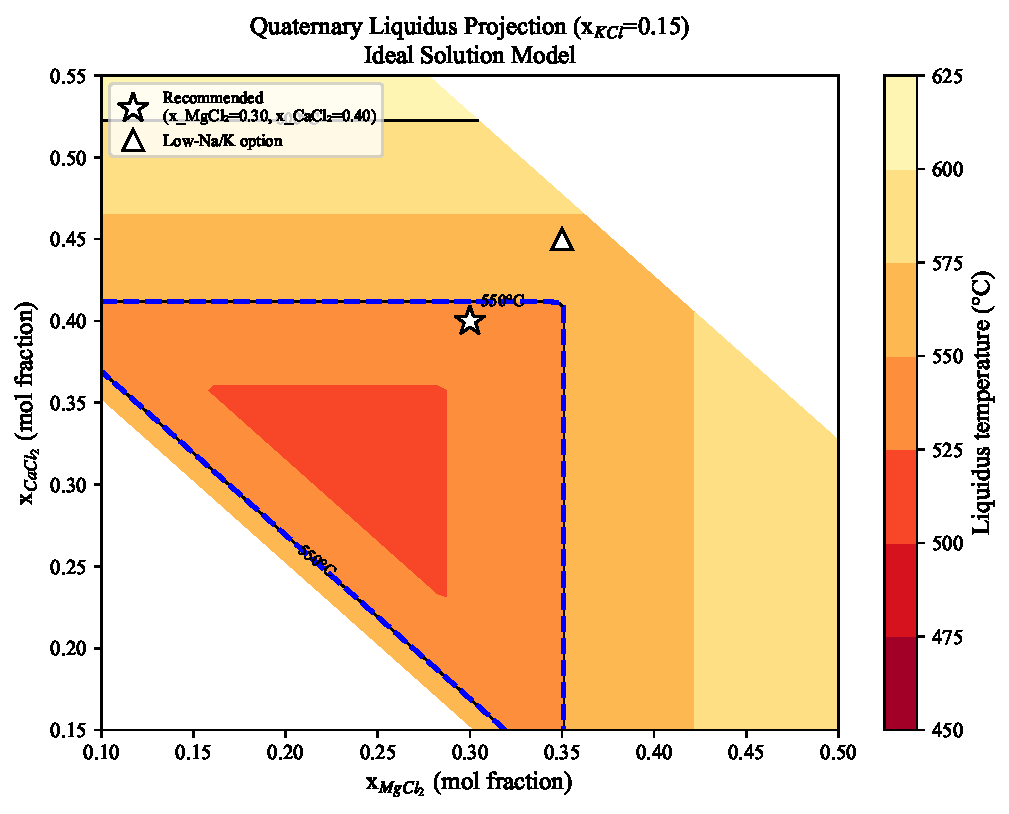
\includegraphics[width=0.95\linewidth]{fig_liquidus.pdf}
\caption{Liquidus projection of the quaternary $\ce{MgCl2-CaCl2-NaCl}$ system at $x_{\ce{KCl}}=0.15$ (ideal solution model).}
\label{fig:liquidus}
\end{figure}

It should be noted that the ideal solution model does not account for solid miscibility gaps or intermediate compounds, and the actual liquidus may deviate substantially. Table~\ref{tab:binary} summarizes the six binary subsystems from the phase-diagram literature \cite{chartrand2000,plettcher1990}: the $\ce{NaCl}$/$\ce{KCl}$-bearing binaries form low-melting compounds/eutectics (minimum liquidus $\sim$440--657~$^{\circ}$C) that \emph{depress} the liquidus, whereas the dominant $\ce{MgCl2-CaCl2}$ pair forms the congruently-melting compound $\ce{CaMg2Cl6}$ ($\approx$621~$^{\circ}$C) that \emph{raises} the liquidus above the ideal prediction. Because $\ce{MgCl2}$+$\ce{CaCl2}$ constitute 70~mol\% of the recommended composition, the net deviation is expected to be upward, consistent with the estimated $\pm$50~$^{\circ}$C uncertainty (upper bound $\sim$594~$^{\circ}$C). Precise prediction requires CALPHAD assessment with dedicated databases (e.g., FactSage SGTE or MTOX); the present calculation serves as a preliminary design guideline. The 36~$^{\circ}$C margin between the calculated liquidus (544~$^{\circ}$C) and the minimum operating temperature (580~$^{\circ}$C) may be insufficient if the actual liquidus exceeds 580~$^{\circ}$C, and a hard operating floor of $\geq$620~$^{\circ}$C (or CALPHAD confirmation of a lower liquidus) is recommended before pilot-scale implementation (see also Limitations~(4)).

\begin{table}[!ht]
\centering
\footnotesize
\caption{Binary subsystems of the quaternary salt and their minimum liquidus features (literature compilation \cite{chartrand2000,plettcher1990}).}
\label{tab:binary}
\begin{tabular}{lcl}
\toprule
Binary system & Key phase(s) & Minimum liquidus ($^{\circ}$C) \\
\midrule
$\ce{MgCl2-NaCl}$ & $\ce{NaMgCl3}$, $\ce{Na2MgCl4}$ & $\sim$440 \\
$\ce{MgCl2-CaCl2}$ & $\ce{CaMg2Cl6}$ (congruent) & $\sim$621 \\
$\ce{CaCl2-NaCl}$ & simple eutectic & $\sim$500 \\
$\ce{CaCl2-KCl}$ & $\ce{KCaCl3}$ + eutectic & $\sim$600 \\
$\ce{MgCl2-KCl}$ & $\ce{KMgCl3}$, $\ce{K2MgCl4}$ & $\sim$470 \\
$\ce{NaCl-KCl}$ & solid solution & $\sim$657 \\
\bottomrule
\end{tabular}
\end{table}

\subsection{Activity Coefficient Sensitivity Analysis}
\label{subsec:activity}

In the quaternary chloride melt, ion-ion interactions cause deviations from ideality ($\gamma \neq 1$). Experimental activity coefficient data for the quaternary $\ce{MgCl2-CaCl2-NaCl-KCl}$ system at 600~$^{\circ}$C are limited in the open literature. Thermodynamic optimization of the $\ce{MgCl2-NaCl}$ binary system \cite{chartrand2000} reports negative deviation ($\gamma < 1$) due to strong $\ce{Mg^{2+}-Cl^{-}}$ interactions. By analogy, $\ce{CaCl2-NaCl}$ and other charge-unsymmetrical chloride mixtures are expected to exhibit similar negative deviation, as established by Kleppa's thermochemical studies of charge-unsymmetrical halide melts \cite{kleppa1966}, though direct activity measurements in the quaternary system remain scarce. The modified quasichemical model (MQM) used in the FactSage Salt database \cite{pelton2000mqm} formally captures these effects, but the database parameters are not publicly available.

To assess the impact of non-ideality on the co-deposition window, a parametric sensitivity analysis is performed. The Nernst equation with activity correction becomes:
\begin{equation}
\label{eq:canernst}
E_{\mathrm{red}}(\ce{Ca^{2+}}) = E^{\circ}_{\mathrm{red}}(\ce{Ca^{2+}/Ca}) + \frac{RT}{2F}\ln(\gamma_{\ce{CaCl2}} \cdot x_{\ce{CaCl2}})
\end{equation}
\begin{equation}
\label{eq:naernst}
E_{\mathrm{red}}(\ce{Na+}) = E^{\circ}_{\mathrm{red}}(\ce{Na+/Na}) + \frac{RT}{F}\ln(\gamma_{\ce{NaCl}} \cdot x_{\ce{NaCl}})
\end{equation}

The co-deposition window $\Delta E = E_{\mathrm{red}}(\ce{Ca^{2+}}) - E_{\mathrm{red}}(\ce{Na+})$ is scanned over $\gamma_{\ce{CaCl2}} = [1.0, 0.9, 0.8, 0.7, 0.5, 0.3]$ and $\gamma_{\ce{NaCl}} = [1.0, 0.85, 0.7]$, covering the range from ideal behavior to strong negative deviation reported for charge-unsymmetrical chloride melts \cite{kleppa1966}. The results (Table~\ref{tab:window_sens}) show that the window remains positive (74.9--147.1~mV) across all 18 combinations, with 15 cases classified as ``Good'' ($>$100~mV) and 3 as ``Moderate'' (50--100~mV). Even at $\gamma_{\ce{CaCl2}} = 0.3$, the narrowest window (74.9~mV, with $\gamma_{\ce{NaCl}} = 1.0$) exceeds the 50~mV threshold for viable co-deposition. The critical $\gamma_{\ce{CaCl2}}$ at which the window vanishes is estimated at $\sim$0.02--0.04 (depending on $\gamma_{\ce{NaCl}}$), far below any physically expected value. This is obtained by setting $\Delta E = 0$ in the Nernst equations (Eqs.~\ref{eq:canernst}--\ref{eq:naernst}), i.e., $E^{\circ}_{\mathrm{red}}(\ce{Ca^{2+}/Ca}) + (RT/2F)\ln(\gamma_{\ce{CaCl2}} \cdot x_{\ce{CaCl2}}) = E^{\circ}_{\mathrm{red}}(\ce{Na+/Na}) + (RT/F)\ln(\gamma_{\ce{NaCl}} \cdot x_{\ce{NaCl}})$, and solving for $\gamma_{\ce{CaCl2}}$ at $T = 873$~K with the recommended composition. The resulting $\gamma_{\ce{CaCl2}} \approx 0.02$--0.04 is far below any physically expected value, indicating that the recommended composition provides a robust co-deposition window even under significant non-ideality, pending CALPHAD validation or direct measurement.

Note that $\gamma_{\ce{CaCl2}}$ and $\gamma_{\ce{NaCl}}$ here denote component-scale activity coefficients of CaCl$_2$ and NaCl, obtained from binary-system measurements \cite{kleppa1966,chartrand2000}. In this work, component-scale activity coefficients are adopted for the Nernst-equation calculation as a feasible approximation, rather than ionic-scale activity coefficients. At high $\ce{CaCl2}$ fractions, the formation of $\ce{CaCl+}$ and $\ce{CaCl3-}$ associates breaks the full-dissociation assumption, which will cause deviation of ionic-scale activity from component-scale activity. This qualitative understanding of Ca--O association is consistent with the short-range-ordering framework adopted in the FactSalt MQM model developed by Pelton et al.\ \cite{pelton2000mqm}, in which ion-pair interactions are considered for molten-salt thermodynamic calculation. This approximation is only used for preliminary evaluation of the co-deposition window, and future MQM-based calculation can separate component activity and ionic activity precisely.

\begin{table}[!ht]
\centering
\footnotesize
\caption{Co-deposition window sensitivity to activity coefficients at 600~$^{\circ}$C}
\label{tab:window_sens}
\begin{tabular}{cccc}
\toprule
$\gamma_{\ce{CaCl2}}$ & $\gamma_{\ce{NaCl}}$ & Window (mV) & Assessment \\
\midrule
1.0 & 1.00 & 120.2 & Good \\
1.0 & 0.85 & 132.4 & Good \\
1.0 & 0.70 & 147.1 & Good \\
0.9 & 1.00 & 116.3 & Good \\
0.9 & 0.85 & 128.5 & Good \\
0.9 & 0.70 & 143.1 & Good \\
0.8 & 1.00 & 111.8 & Good \\
0.8 & 0.85 & 124.1 & Good \\
0.8 & 0.70 & 138.7 & Good \\
0.7 & 1.00 & 106.8 & Good \\
0.7 & 0.85 & 119.0 & Good \\
0.7 & 0.70 & 133.6 & Good \\
0.5 & 1.00 & 94.2 & Moderate \\
0.5 & 0.85 & 106.4 & Good \\
0.5 & 0.70 & 121.0 & Good \\
0.3 & 1.00 & 74.9 & Moderate \\
0.3 & 0.85 & 87.2 & Moderate \\
0.3 & 0.70 & 101.8 & Good \\
\bottomrule
\end{tabular}
\end{table}

\subsection{Mg--Ca Liquid Alloy Thermodynamic Parameters}
\label{subsec:MgCa}

The in-situ co-deposited Mg--Ca forms a liquid alloy at 600~$^{\circ}$C (above the Mg--Ca eutectic at $\approx$517~$^{\circ}$C). The Mg--Ca system has been assessed by Nayeb-Hashemi and Clark \cite{nayeb1988} and re-assessed by Zhang et al. \cite{zhang2008mgce} using the CALPHAD method. The liquid phase is described by a Redlich--Kister expansion:
\begin{equation}
\label{eq:rk}
G^{\mathrm{ex}}_{\mathrm{Mg-Ca}} = x_{\mathrm{Mg}}x_{\mathrm{Ca}}\left[L_0 + L_1(x_{\mathrm{Mg}}-x_{\mathrm{Ca}})\right]
\end{equation}
The formation of the stable intermetallic $\ce{Mg2Ca}$ indicates exothermic mixing. Zhang et al. \cite{zhang2008mgce} reported Redlich--Kister parameters $L_0 = -30616 + 13.72\,T$~J/mol and $L_1 = -532 + 2.70\,T$~J/mol for the liquid phase. At 600~$^{\circ}$C (873~K), $L_0 = -18.64$~kJ/mol. Using a regular solution approximation ($L_1 = 0$, $\Omega \approx L_0$), the mixing enthalpy at equimolar composition is $-4.66$~kJ/mol, consistent with the assessed phase diagram and the $\ce{Mg2Ca}$ intermetallic formation energy.

At 600~$^{\circ}$C (873~K), the mixing thermodynamics are:
\begin{equation}
\label{eq:mix}
\Delta G_{\mathrm{mix}} = RT(x_{\mathrm{Mg}}\ln x_{\mathrm{Mg}} + x_{\mathrm{Ca}}\ln x_{\mathrm{Ca}}) + \Omega\,x_{\mathrm{Mg}}x_{\mathrm{Ca}}
\end{equation}
At equimolar composition: $\Delta G_{\mathrm{mix}} = -9.69$~kJ/mol, $\Delta H_{\mathrm{mix}} = -4.66$~kJ/mol, $\Delta S_{\mathrm{mix}} = 5.76$~J/(mol$\cdot$K), and activity coefficients $\gamma_{\mathrm{Mg(alloy)}} = \gamma_{\mathrm{Ca(alloy)}} = 0.526$. The negative $\Delta G_{\mathrm{mix}}$ indicates spontaneous alloy formation, suggesting homogeneous Mg--Ca co-deposition at the cathode. The strong negative deviation ($\gamma \ll 1$) suggests that the Mg--Ca liquid alloy is thermodynamically stable, which is favorable for sustained complementary reduction. The regular solution approximation ($L_1 = 0$) introduces a minor deviation: at equimolar composition, the neglected $L_1$ term contributes $L_1 \cdot (x_{\mathrm{Mg}} - x_{\mathrm{Ca}}) \cdot x_{\mathrm{Mg}} x_{\mathrm{Ca}} = 0$ at $x = 0.5$ (since $x_{\mathrm{Mg}} - x_{\mathrm{Ca}} = 0$), and the maximum deviation occurs off-equimolar compositions at $<$1~kJ/mol, which does not affect the qualitative conclusion of spontaneous mixing. Additionally, the regular-solution approximation neglects ordering effects associated with the stable $\ce{Mg2Ca}$ intermetallic; the resulting $\Delta G_{\mathrm{mix}}$ uncertainty is estimated at $\pm$2--3~kJ/mol near the $\ce{Mg2Ca}$ stoichiometry, but the qualitative conclusion of spontaneous alloy formation remains valid.

\section{Results and Discussion}

\subsection{Reduction Thermodynamics and Deoxidation Limits}

Table~\ref{tab:thermo} presents the calculated $\Delta G^{\circ}$ and $\Delta H^{\circ}$ for three reduction pathways at 550--650~$^{\circ}$C.

\begin{table}[!ht]
\centering
\footnotesize
\caption{$\Delta G^{\circ}$ and $\Delta H^{\circ}$ of reduction reactions (kJ/mol)}
\label{tab:thermo}
\begin{tabular}{lccc}
\toprule
\multirow{2}{*}{Reaction} & \multicolumn{3}{c}{$\Delta G^{\circ}\;/\;\Delta H^{\circ}$} \\
\cmidrule(lr){2-4}
 & 550~$^{\circ}$C & 600~$^{\circ}$C & 650~$^{\circ}$C \\
\midrule
$\ce{TiO2 + 2Mg -> Ti + 2MgO}$ & $-232.7/-259.8$ & $-231.0/-260.0$ & $-229.4/-260.1$ \\
$\ce{TiO2 + 2Ca -> Ti + 2CaO}$ & $-308.4/-322.9$ & $-307.5/-322.6$ & $-306.6/-322.2$ \\
$\ce{TiO2 + Mg + Ca -> Ti + MgO + CaO}$ & $-270.5/-291.4$ & $-269.3/-291.3$ & $-268.0/-291.2$ \\
\bottomrule
\end{tabular}
\end{table}

All three pathways are strongly exergonic ($\Delta G^{\circ} = -231.0$ to $-307.5$~kJ/mol at 600~$^{\circ}$C), indicating thermodynamic feasibility. The Ca reduction is 76.5~kJ/mol more negative than Mg, demonstrating Ca's stronger deoxidation driving force. The exothermic nature ($\Delta H^{\circ} = -260$ to $-323$~kJ/mol) partially compensates for electrolysis heat losses.

The equilibrium oxygen content in titanium is calculated using the dissolution free energy of oxygen in $\alpha$-Ti, $\Delta G^{\circ}_{\mathrm{diss}}(\mathrm{O\;in\;\alpha\text{-}Ti}) \approx -581{,}000 + 92T$ (J/mol, standard state: 1~wt\% Henry's law) \cite{waldner1999}. The deoxidation free energy is:
\begin{equation}
\label{eq:deox}
\Delta G^{\circ}_{\mathrm{deox}} = \Delta G^{\circ}_{f}(\mathrm{MO}) - \Delta G^{\circ}_{\mathrm{diss}}(\mathrm{O\;in\;\alpha\text{-}Ti})
\end{equation}
where both terms are on a 1~mol O basis: $\Delta G^{\circ}_{f}(\mathrm{MO})$ is the formation free energy for $\mathrm{M} + \tfrac{1}{2}\ce{O2} \to \mathrm{MO}$ (per mol MO, containing 1~mol O), and $\Delta G^{\circ}_{\mathrm{diss}}$ is the dissolution free energy for $\tfrac{1}{2}\ce{O2} \to [\mathrm{O}]_{\mathrm{Ti}}$ (negative, spontaneous dissolution). The equilibrium constant $K = \exp(-\Delta G^{\circ}_{\mathrm{deox}}/RT)$ yields $w_{[\mathrm{O}]} = 1/K$ (Henry's law, dilute solution). At 600~$^{\circ}$C, Mg deoxidation yields 3908~ppm O while Ca reaches 20~ppm---a 194$\times$ difference (Table~\ref{tab:deox}). This quantitatively justifies the bimetallic strategy: Mg performs bulk reduction ($\sim$40~wt\% $\to \sim$0.4~wt\% O), while Ca polishes far below the 0.10--0.20~wt\% target (to $\sim$20~ppm). When the Mg--Ca alloy activity ($a_M = \gamma_{\mathrm{alloy}} \cdot x_M = 0.526 \times 0.5 = 0.263$) is accounted for, both equilibrium oxygen levels increase by a factor of $\sim$3.8 ($\sim$14{,}900~ppm for Mg, $\sim$77~ppm for Ca), but the 194$\times$ ratio is preserved, confirming that the bimetallic strategy remains effective even under alloy conditions. It should be emphasized that $a_M = 0.263$ is a \emph{global} equimolar average; in a real in-situ co-deposition the cathode-surface alloy composition varies spatially and temporally (locally Ca-rich or Mg-rich regions), so the local equilibrium oxygen content is inhomogeneous and is bounded by the pure-metal columns of Table~\ref{tab:deox} (pure Mg: 3908~ppm; pure Ca: 20~ppm). Achieving a uniform final oxygen content therefore requires sufficient melt convection and mixing of the co-deposited metals, a point that merits experimental attention. The temperature-dependent dissolution free energy $\Delta G^{\circ}_{\mathrm{diss}} \approx -581{,}000 + 92T$~J/mol is derived from the CALPHAD assessment of the Ti--O system \cite{waldner1999}, which is validated for the $\alpha$-Ti phase field ($<$882~$^{\circ}$C). Across the operating window of 580--650~$^{\circ}$C the equilibrium oxygen content shifts by roughly $\sim$30\% (Mg) to a factor of $\sim$2 (Ca) (Table~\ref{tab:deox}); because Ca remains $\sim$100$\times$ deeper than Mg throughout this window, the order-of-magnitude conclusion is unaffected.

\begin{table}[!ht]
\centering
\footnotesize
\caption{Equilibrium oxygen content in titanium. Columns ``$a_M=1$'' assume pure metal; columns ``$a_M=0.263$'' account for the Mg--Ca liquid alloy activity ($\gamma_{\mathrm{alloy}}=0.526$, $x_M=0.5$).}
\label{tab:deox}
\begin{tabular}{lccccc}
\toprule
Deoxidant/T & $\Delta G^{\circ}_{\mathrm{deox}}$ & $w_{[\mathrm{O}]}^{\mathrm{eq}}$ & $w_{[\mathrm{O}]}^{\mathrm{eq}}$ & $w_{[\mathrm{O}]}^{\mathrm{eq}}$ & $w_{[\mathrm{O}]}^{\mathrm{eq}}$ \\
 & (kJ/mol) & \multicolumn{2}{c}{$a_M=1$ (pure)} & \multicolumn{2}{c}{$a_M=0.263$ (alloy)} \\
\cmidrule(lr){3-4} \cmidrule(lr){5-6}
 & & (wt\%) & (ppm) & (wt\%) & (ppm) \\
\midrule
Mg / 550~$^{\circ}$C & $-7.5$ & 0.333 & 3325 & 1.264 & 12643 \\
Mg / 600~$^{\circ}$C & $-6.8$ & 0.391 & 3908 & 1.486 & 14859 \\
Mg / 650~$^{\circ}$C & $-6.1$ & 0.451 & 4510 & 1.715 & 17146 \\
Ca / 550~$^{\circ}$C & $-45.4$ & 0.0013 & 13.2 & 0.0050 & 50.2 \\
Ca / 600~$^{\circ}$C & $-45.0$ & 0.0020 & 20.2 & 0.0077 & 76.8 \\
Ca / 650~$^{\circ}$C & $-44.7$ & 0.0029 & 29.4 & 0.0112 & 111.8 \\
\bottomrule
\end{tabular}
\end{table}

\subsection{$\ce{Ca^{2+}/Na+}$ Co-Deposition Window}

Table~\ref{tab:Ed} lists the standard decomposition voltages ($E_d$) and the corresponding reduction potentials ($E^{\circ}_{\mathrm{red}} = -E_d$) of the four pure chlorides at 600~$^{\circ}$C, all referenced to the $\ce{Cl2/Cl-}$ electrode.

\begin{table}[!ht]
\centering
\footnotesize
\caption{Decomposition voltages and reduction potentials of pure chlorides at 600~$^{\circ}$C (vs.\ $\ce{Cl2/Cl-}$). Note: $n$ denotes the number of electrons transferred per formula unit ($n = z_{\mathrm{cation}}$); $\Delta G^{\circ}_f$ values are Kirchhoff-corrected to 873~K from Barin \cite{barin1995}; $E_d = -\Delta G^{\circ}_f/(nF)$.}
\label{tab:Ed}
\begin{tabular}{lccc}
\toprule
Chloride & $\Delta G^{\circ}_f$ (kJ/mol) & $E_d$ (V) & $E^{\circ}_{\mathrm{red}}$ (V) \\
\midrule
$\ce{MgCl2}$ & $-501.9$ & 2.601 & $-2.601$ \\
$\ce{NaCl}$  & $-331.9$ & 3.440 & $-3.440$ \\
$\ce{CaCl2}$ & $-661.5$ & 3.428 & $-3.428$ \\
$\ce{KCl}$   & $-354.6$ & 3.675 & $-3.675$ \\
\bottomrule
\end{tabular}
\end{table}

Among the pure salts, $\ce{Mg^{2+}}$ is the easiest to reduce ($E^{\circ}_{\mathrm{red}} = -2.601$~V), while $\ce{K+}$ is the hardest ($-3.675$~V). Critically, $\ce{Ca^{2+}}$ and $\ce{Na+}$ have nearly identical reduction potentials in pure salts: $E^{\circ}_{\mathrm{red}}(\ce{Ca^{2+}/Ca}) - E^{\circ}_{\mathrm{red}}(\ce{Na+/Na}) = +12$~mV, meaning $\ce{Ca^{2+}}$ is marginally easier to reduce in pure salts. This $\pm$12~mV gap is within the $\approx\pm$2~kJ/mol uncertainty of the underlying $\Delta G^{\circ}_f$ data (Sec.~\ref{subsec:data}), which translates to $\approx\pm$20~mV for a monovalent chloride; the intrinsic Ca/Na preference is therefore weak, and the practical co-deposition selectivity is dominated by the concentration ratio ($x_{\ce{CaCl2}}/x_{\ce{NaCl}} = 0.40/0.15$) rather than by the intrinsic potential difference. The Downs process operates with a $\ce{CaCl2}$-majority electrolyte ($\sim$67~wt\% $\ce{CaCl2}$ / 33~wt\% $\ce{NaCl}$, roughly equimolar on a molar basis), yet deposits Na, because $\ce{Ca^{2+}}$ reduction is kinetically inhibited (large activation overpotential) relative to $\ce{Na+}$. The pure-salt near-identical potentials thus bear only superficial similarity to the Downs process: the Downs selectivity is \emph{kinetic} in origin, whereas the present $\ce{CaCl2}$-rich composition ($x_{\ce{CaCl2}}/x_{\ce{NaCl}} = 0.40/0.15$) adds a $\sim$120~mV \emph{thermodynamic} bias favoring Ca.

In the recommended quaternary composition ($x_{\ce{MgCl2}}=0.30$, $x_{\ce{CaCl2}}=0.40$, $x_{\ce{NaCl}}=0.15$, $x_{\ce{KCl}}=0.15$), Nernst concentration correction shifts the effective reduction potentials. The Nernst-corrected window $\Delta E = E_{\mathrm{red}}(\ce{Ca^{2+}}) - E_{\mathrm{red}}(\ce{Na+})$ becomes +120~mV under the ideal solution assumption (calculated using the $E^{\circ}_{\mathrm{red}}$ values from Table~\ref{tab:Ed} at 600~$^{\circ}$C), meaning $\ce{Ca^{2+}}$ now reduces before $\ce{Na+}$. As shown in Section~\ref{subsec:activity}, the activity coefficient sensitivity analysis supports that this window remains positive (74.9--147.1~mV) across all 18 tested $\gamma$ combinations ($\gamma_{\ce{CaCl2}} = 0.3$--1.0), suggesting the robustness of the composition design.

The above window is an \emph{equilibrium} quantity. Under polarization, the effective deposition potentials shift by the activation overpotential $\eta_{\mathrm{act}} = (RT/\alpha nF)\,\mathrm{asinh}(j/2j_0)$, where $j$ is the current density and $j_0$ the exchange current density. Adopting order-of-magnitude $j_0$ values typical of metal deposition in chloride melts ($j_0^{\mathrm{Ca}}\approx 0.05$~A/cm$^2$, $j_0^{\mathrm{Na}}\approx 0.03$~A/cm$^2$, transfer coefficient $\alpha = 0.5$) \cite{plettcher1990}, the activation overpotential of the monovalent $\ce{Na+}$ grows far faster than that of the divalent $\ce{Ca^{2+}}$ (Fig.~\ref{fig:overpotential}): at $j = 0.5$~A/cm$^2$, $\eta_{\mathrm{act}}^{\mathrm{Ca}} \approx 174$~mV versus $\eta_{\mathrm{act}}^{\mathrm{Na}} \approx 424$~mV. The effective window $E_{\mathrm{eff}}(\ce{Ca^{2+}}) - E_{\mathrm{eff}}(\ce{Na+}) = \Delta E + (\eta_{\mathrm{Na}} - \eta_{\mathrm{Ca}})$ therefore \emph{widens} from 120~mV (equilibrium) to $\sim$370~mV at $j = 0.5$~A/cm$^2$, and to $\sim$470~mV at $j = 2$~A/cm$^2$. Kinetic polarization thus favors Ca co-deposition, but this estimate is qualitative and its sign is not established: the assumed $j_0^{\mathrm{Ca}} > j_0^{\mathrm{Na}}$ favors Ca, yet the Downs cell deposits Na from a $\ce{CaCl2}$-majority melt, indicating that $\ce{Ca^{2+}}$ reduction may instead be kinetically \emph{slower}, which would \emph{narrow} rather than widen the practical window. The $j_0$ and $\alpha$ values for the quaternary melt are unknown and require cyclic-voltammetry measurement, so the direction of the kinetic correction must be established before the enlarged window of Fig.~\ref{fig:overpotential} can be relied upon; concentration polarization at very high $j$ could additionally reverse the trend by depleting $\ce{Ca^{2+}}$ at the cathode.

\begin{figure}[!ht]
\centering
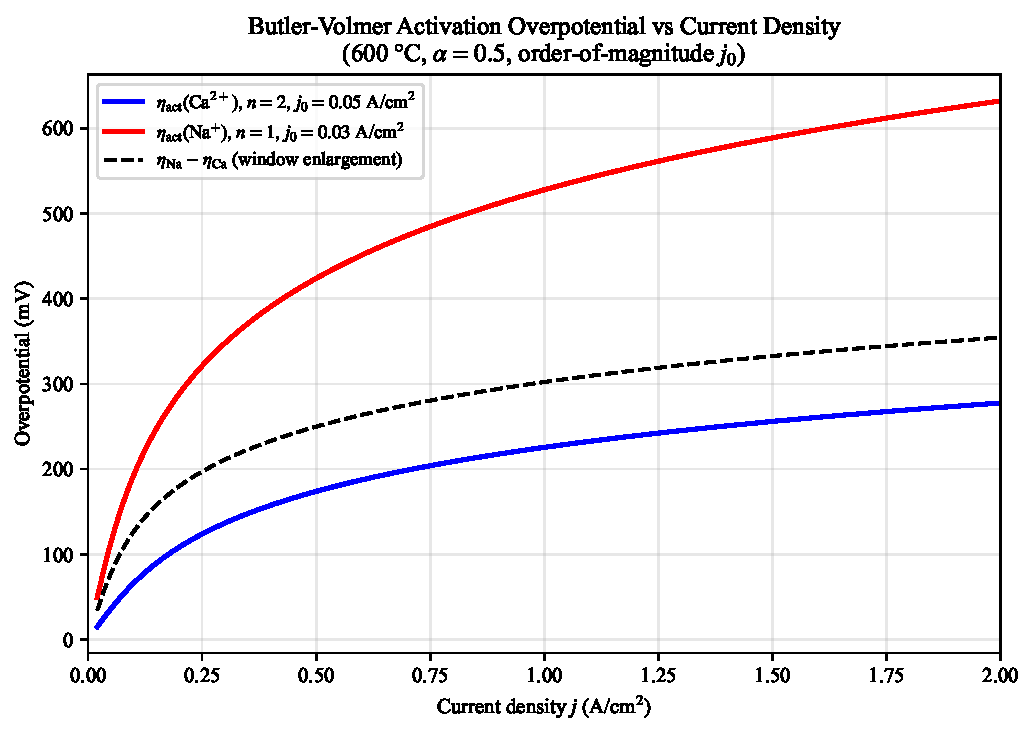
\includegraphics[width=0.85\linewidth]{fig_overpotential_bv.pdf}
\caption{Butler--Volmer activation overpotentials of $\ce{Ca^{2+}}$ ($n=2$) and $\ce{Na+}$ ($n=1$) versus current density at 600~$^{\circ}$C ($\alpha=0.5$, order-of-magnitude $j_0$). The dashed line is the kinetic enlargement of the co-deposition window, $\eta_{\mathrm{Na}} - \eta_{\mathrm{Ca}}$.}
\label{fig:overpotential}
\end{figure}

\emph{Mg/Ca co-deposition ratio.} The analysis above concerns only the $\ce{Ca^{2+}/Na+}$ selectivity. The far larger $\ce{Mg^{2+}/Ca^{2+}}$ gap is not addressed by the equilibrium window: at the recommended composition ($x_{\ce{MgCl2}}=0.30$, $x_{\ce{CaCl2}}=0.40$), the Nernst-corrected potentials give $E_{\mathrm{red}}(\ce{Ca^{2+}}) - E_{\mathrm{red}}(\ce{Mg^{2+}}) \approx -816$~mV, i.e., Mg reduces $\sim$816~mV earlier than Ca. The equimolar Mg--Ca alloy assumed in Sec.~\ref{subsec:MgCa} and in the material balance (Table~\ref{tab:mbalance}) is therefore \emph{not} a thermodynamic outcome: it can only be approached when Mg deposition reaches its mass-transfer (diffusion) limit at the cathode, after which Ca co-deposits, as in conventional alloy co-deposition (e.g., Zn--Ni, Li--Na). The actual Mg/Ca ratio is thus set by the operating current density relative to the Mg limiting current density---a design variable requiring experimental determination---and the 1:1 assumption should be regarded as a bounding idealization.

\subsection{E--$p\ce{O^{2-}}$ Stability Diagram and Impurity Separation}

The E--$p\ce{O^{2-}}$ diagram (Fig.~\ref{fig:EpO2}) plots the M/MO equilibrium lines according to:
\begin{equation}
\label{eq:epo2}
E = E^{\circ}_{\mathrm{red}} + \frac{RT}{2F}\ln(10)\cdot p\ce{O^{2-}}
\end{equation}
where $p\ce{O^{2-}} = -\log_{10}(a_{\ce{O^{2-}}})$ and $E^{\circ}_{\mathrm{red}} = \Delta G^{\circ}_{f,\mathrm{MO}}/(nF)$ is the standard reduction potential referenced to the $\ce{O2/O^{2-}}$ couple ($p_{\ce{O2}}=1$~atm, $a_{\ce{O^{2-}}}=1$), with $n = 2$ electrons transferred per $\ce{O^{2-}}$ in the oxide formula unit ($n=4$ for $\ce{TiO2}$ and $\ce{SiO2}$, $n=6$ for $\ce{Fe2O3}$ and $\ce{Al2O3}$, $n=2$ for $\ce{MgO}$ and $\ce{CaO}$). The derivation proceeds as follows: for a divalent-oxide half-reaction $\ce{MO + 2e^- -> M + O^{2-}}$, the Nernst equation gives $E = E^{\circ}_{\mathrm{red}} - (RT/2F)\ln(a_{\ce{O^{2-}}})$; substituting $\ln(a_{\ce{O^{2-}}}) = -\ln(10)\cdot p\ce{O^{2-}}$ yields the above equation with a positive slope. The Nernst slope at 600~$^{\circ}$C is 86.6~mV per $p\ce{O^{2-}}$ unit.

\begin{figure}[!ht]
\centering
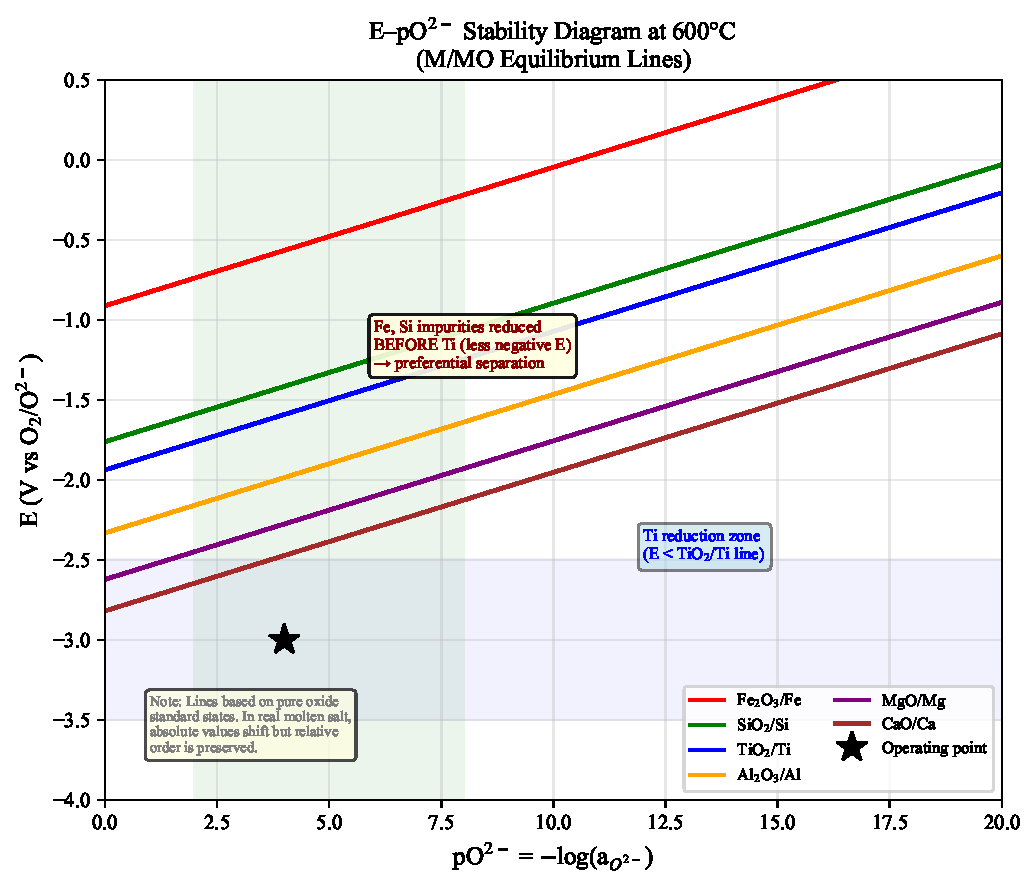
\includegraphics[width=0.95\linewidth]{fig_E_pO2.pdf}
\caption{E--$p\ce{O^{2-}}$ stability diagram at 600~$^{\circ}$C. All potentials are referenced to the $\ce{O2/O^{2-}}$ electrode ($p_{\ce{O2}}=1$~atm, $a_{\ce{O^{2-}}}=1$), not the $\ce{Cl2/Cl-}$ electrode used in Table~\ref{tab:Ed}. Lines based on pure oxide standard states; in real molten salt, $\ce{Ca^{2+}}$--$\ce{O^{2-}}$ complexation lowers $a_{\ce{O^{2-}}}$, shifting all potentials positively, but the relative reduction order ($\ce{Fe2O3} > \ce{SiO2} > \ce{TiO2} > \ce{Al2O3} > \ce{MgO} > \ce{CaO}$) is preserved.}
\label{fig:EpO2}
\end{figure}

The reduction potentials follow: $\ce{Fe2O3}$ ($-1.01$~V) $>$ $\ce{SiO2}$ ($-1.95$~V) $>$ $\ce{TiO2}$ ($-2.03$~V) $>$ $\ce{Al2O3}$ ($-2.42$~V) $>$ $\ce{MgO}$ $>$ $\ce{CaO}$, indicating that Fe and Si impurities reduce before Ti. This thermodynamic preferential reduction, combined with density differences (Fe: 7.87~g/cm$^3$ vs.\ Ti: 4.51~g/cm$^3$), suggests a potential pathway for physical separation of impurity metals from titanium powder. However, it should be noted that the Fe--Ti and Si--Ti systems exhibit extensive solid solubility and form intermetallic compounds (e.g., FeTi, $\ce{Fe2Ti}$, $\ce{Ti5Si3}$, $\ce{TiSi2}$) at 600~$^{\circ}$C, which may complicate gravity-based separation. The use of metallurgical-grade $\ce{TiO2}$ ($\geq$90~wt\%) thus requires further investigation of impurity phase distribution and may need complementary separation strategies (e.g., acid leaching). This thermodynamic basis indicates potential compatibility with metallurgical-grade $\ce{TiO2}$, subject to kinetic and purity validation. Notably, because $\ce{Ca^{2+}}$ exhibits stronger complexation with $\ce{O^{2-}}$ than $\ce{Mg^{2+}}$ does, the activity coefficient of dissolved CaO is suppressed more significantly than that of MgO. This differential non-ideality suggests that in a real chloride--oxide melt, the difference between CaO and MgO reduction potentials may be larger than predicted from pure-oxide standard states. Such a shift would be favorable for the proposed complementary mechanism, reinforcing the sequential roles of Mg for rapid bulk reduction and Ca for deep deoxidation.

\subsection{SCM Kinetics and Parameter Sensitivity}
\label{subsec:scm}

The reduction kinetics are modeled using the shrinking core model (SCM) with diffusion control through the porous Ti product layer \cite{levenspiel1999}:
\begin{equation}
\label{eq:scm}
t_{\mathrm{complete}} = \frac{c_{[\mathrm{O}]\in\ce{TiO2}} \cdot R^2}{6\,D_{\mathrm{eff}}\,c_{\mathrm{red}}}
\end{equation}
where $c_{[\mathrm{O}]\in\ce{TiO2}} \approx 1.06\times10^5$~mol/m$^3$ (oxygen concentration in $\ce{TiO2}$), $c_{\mathrm{red}} \approx 635$~mol/m$^3$ (estimated from 3~mol\% dissolved Mg/Ca in the melt, assuming a melt density of $\sim$1.8~g/cm$^3$ at 600~$^{\circ}$C \cite{sato1999} and an effective molar mass $M_{\mathrm{avg}} \approx 85$~g/mol, giving $c_{\mathrm{red}} \approx 0.03 \times 1.8\times10^3 / (85\times10^{-3}) \approx 635$~mol/m$^3$), and $D_{\mathrm{eff}} = D \cdot \varepsilon/\tau$ with porosity $\varepsilon = 0.3$ and tortuosity $\tau = 3.0$ (typical values for porous metallic product layers \cite{fray2000}). Here $D$ denotes the intrinsic diffusivity of the rate-limiting species through the porous Ti layer, and $D_{\mathrm{eff}}$ is the effective diffusivity accounting for porosity and tortuosity. Two possible rate-limiting mechanisms exist in this chemical reduction system: outward diffusion of O$^{2-}$ through the Ti product layer, or inward diffusion of Mg/Ca toward the unreduced core. In this work, $D = 2.0\times10^{-9}$~m$^2$/s is adopted as a representative value, consistent with measured O$^{2-}$ diffusivities of $\sim$1--3$\times10^{-9}$~m$^2$/s in molten $\ce{CaCl2}$-based FFC melts \cite{fray2000,yan2007}; the actual rate-limiting species (O$^{2-}$ outward vs.\ Mg/Ca inward) requires further study. Using these parameters, 100~$\mu$m-diameter particles ($R = 50~\mu$m) require 5.8~min for complete reduction (Fig.~\ref{fig:scm}).

\begin{figure}[!ht]
\centering
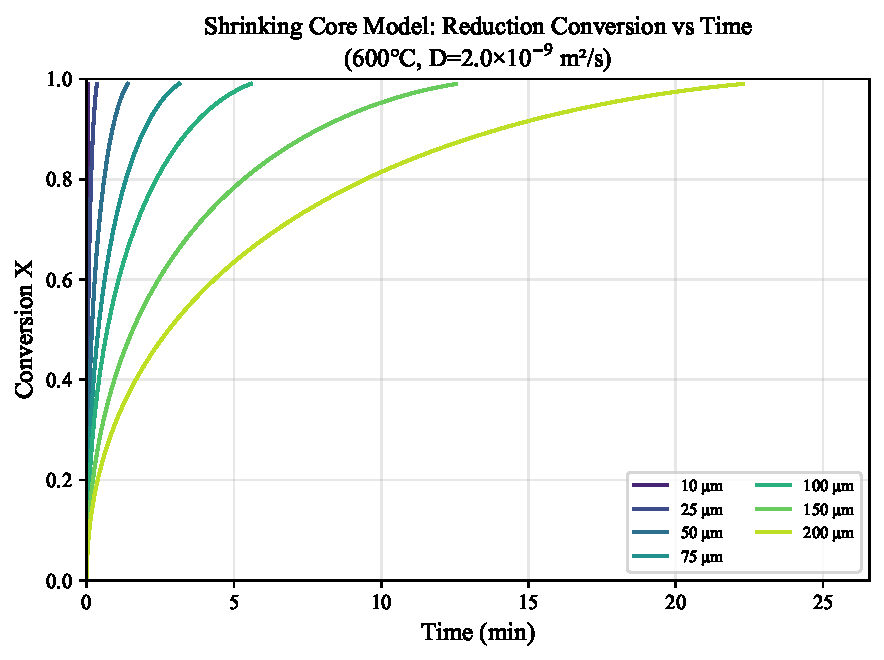
\includegraphics[width=0.95\linewidth]{fig_scm_conversion.pdf}
\caption{SCM-predicted conversion versus time for different particle sizes ($D = 2.0\times10^{-9}$~m$^2$/s, 600~$^{\circ}$C).}
\label{fig:scm}
\end{figure}

A sensitivity analysis over $D = 1.0$--$3.0\times10^{-9}$~m$^2$/s (Fig.~\ref{fig:scm_sens}) shows that 100~$\mu$m-diameter particle reduction time ranges from 3.9~min ($D=3.0\times10^{-9}$) to 11.6~min ($D=1.0\times10^{-9}$), with the nominal 5.8~min falling within this range. The complete reduction time as a function of particle diameter is shown in Fig.~\ref{fig:scm_time}, illustrating the inverse-square scaling. Additional sensitivity to $\varepsilon$ (0.1--0.5) and $\tau$ (1.5--5.0) yields a broader $D_{\mathrm{eff}}$ range of $0.2\times10^{-10}$--$10\times10^{-10}$~m$^2$/s, corresponding to 1.2--58~min, indicating that precise prediction requires determination of product-layer microstructure.

It is important to note that the above $D$ range ($10^{-9}$~m$^2$/s) corresponds to the \emph{chemical diffusion control} mechanism, where the rate-limiting step is liquid-phase diffusion of Mg/Ca through the porous Ti layer. If the actual rate-limiting mechanism were \emph{solid-state diffusion} of O$^{2-}$ through the Ti product layer, $D$ could be 2--3 orders of magnitude lower ($\sim$10$^{-12}$--10$^{-10}$~m$^2$/s), yielding reduction times of $\sim$2--193~hours for 100~$\mu$m particles. This would make the process impractical for single-step batch reduction. The present process must therefore rely on the chemical diffusion mechanism, which is plausible given that the co-deposited Mg--Ca alloy is liquid at 600~$^{\circ}$C (the Mg--Ca eutectic is $\approx$517~$^{\circ}$C, Sec.~\ref{subsec:MgCa}), so the reductant can permeate the porous product layer as a liquid phase, but this mechanistic assumption requires experimental confirmation. Furthermore, the SCM model assumes internal (pore) diffusion through the product layer as the rate-limiting step. External film diffusion around the particle could become rate-limiting at very high flow rates or very small particle sizes ($<$10~$\mu$m), but for the 25--100~$\mu$m particle range of interest and typical melt agitation conditions, the internal diffusion resistance is expected to dominate by 1--2 orders of magnitude based on the Sherwood number criterion ($\mathrm{Sh} \gg 1$). A quantitative comparison of internal vs.\ external diffusion resistances requires melt hydrodynamic data (stirring speed, viscosity) that are not available at the conceptual design stage.

To propagate uncertainties globally, a Monte Carlo simulation ($N = 10^5$, fixed random seed $= 42$ for reproducibility) was performed with the five uncertain parameters sampled simultaneously: $D \sim U(1, 3) \times 10^{-9}$~m$^2$/s, $\varepsilon \sim U(0.1, 0.5)$, $\tau \sim U(1.5, 5.0)$, $\eta_I \sim \mathrm{Tri}(0.50, 0.75, 0.88)$, and $V_{\mathrm{cell}} \sim \mathcal{N}(4.1, 0.3)$ truncated to [3.5, 4.5]~V. The $\eta_I$ distribution spans 0.50--0.88 so that the analysis encompasses both the target range and the worst-case FFC-like scenario ($\eta_I = 0.50$--0.60) without presupposing the feasibility threshold. The distributions for $\varepsilon$ and $\tau$ are based on typical ranges for porous metallic product layers reported in the FFC and powder metallurgy literature \cite{fray2000}; these parameters are treated as static uncertainty intervals for sensitivity analysis. The results (Fig.~\ref{fig:monte_carlo}) show that the SCM reduction time follows a lognormal distribution with median 6.6~min (P5--P95: 2.5--19.9~min), while the net energy consumption follows a right-skewed distribution with median 11{,}781~kWh/ton-Ti (P5--P95: 9{,}515--15{,}362~kWh/ton-Ti). The probability of achieving $W_{\mathrm{net}} < 11{,}192$~kWh/ton-Ti (the nominal value) is 35.8\%, and $P(W_{\mathrm{net}} < 14{,}000) = 85.8\%$. For comparison, $P(W_{\mathrm{net}} < 16{,}000) \approx 97\%$ and $P(W_{\mathrm{net}} < 20{,}000) \approx 100\%$. The second-law efficiency (based on 4{,}550~kWh/ton-Ti reversible work) has a mean of 38.6\% (P5--P95: 29.6--47.8\%). Spearman rank correlation analysis (Fig.~\ref{fig:tornado}) reveals that $\eta_I$ ($\rho = -0.85$) dominates energy uncertainty, followed by $V_{\mathrm{cell}}$ ($\rho = 0.50$); for SCM time, $\varepsilon$ ($\rho = -0.68$) and $\tau$ ($\rho = 0.52$) are the dominant parameters. The energy feasibility conclusion is therefore highly sensitive to the $\eta_I$ assumption, and experimental validation of current efficiency is the most critical prerequisite for process viability. It should be noted that the present Monte Carlo analysis does not include uncertainties in $\gamma_{\ce{CaCl2}}$, liquidus temperature, or oxide solubility; a more comprehensive global uncertainty analysis incorporating these thermochemical parameters is recommended for future work. Semi-quantitatively, these omitted terms act on \emph{feasibility} rather than on the energy figure: (i) the $\gamma_{\ce{CaCl2}} = 0.3$--1.0 scan (Table~\ref{tab:window_sens}) changes the co-deposition window by $\sim$60--75~mV but never closes it, so it does not materially perturb the energy estimate; (ii) the liquidus uncertainty ($\pm$50~$^{\circ}$C) instead constrains the \emph{operable} temperature, hence the process viability (Limitations~(4)); and (iii) the oxide-solubility uncertainty (0.5--1.2~wt\%) changes the required salt inventory by a factor of 2--4 (Sec.~\ref{subsec:dissolution}), which affects capital cost and closed-loop feasibility far more than it affects the per-ton energy. The energy prediction is therefore dominated by $\eta_I$ (as the Spearman analysis shows), whereas process \emph{feasibility} is governed more critically by the 600~$^{\circ}$C oxide solubility and the liquidus.

\begin{figure}[!htbp]
\centering
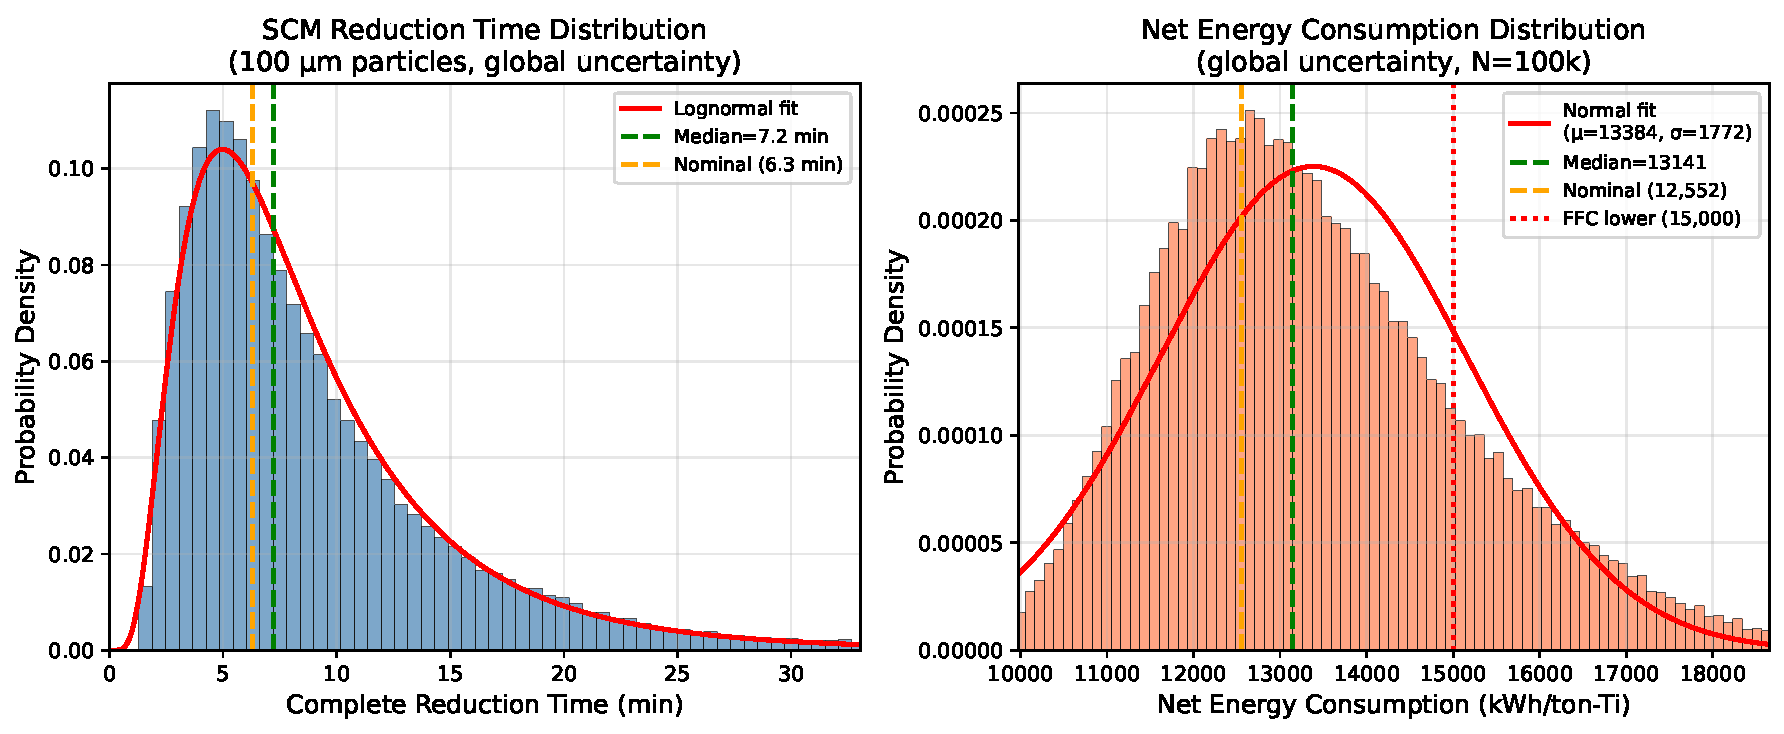
\includegraphics[width=0.95\linewidth]{fig_monte_carlo.pdf}
\caption{Monte Carlo global uncertainty analysis ($N = 10^5$): (left) SCM reduction time distribution with lognormal fit; (right) net energy consumption distribution. Dashed lines indicate nominal values. The analysis simultaneously sampled five parameters: diffusion coefficient $D$, porosity $\varepsilon$, tortuosity $\tau$, current efficiency $\eta_I \sim \mathrm{Tri}(0.50, 0.75, 0.88)$, and cell voltage $V_{\mathrm{cell}} \sim \mathcal{N}(4.1, 0.3)$. The $\eta_I$ lower bound of 0.50 encompasses the worst-case FFC-like scenario.}
\label{fig:monte_carlo}
\end{figure}

\begin{figure}[!htbp]
\centering
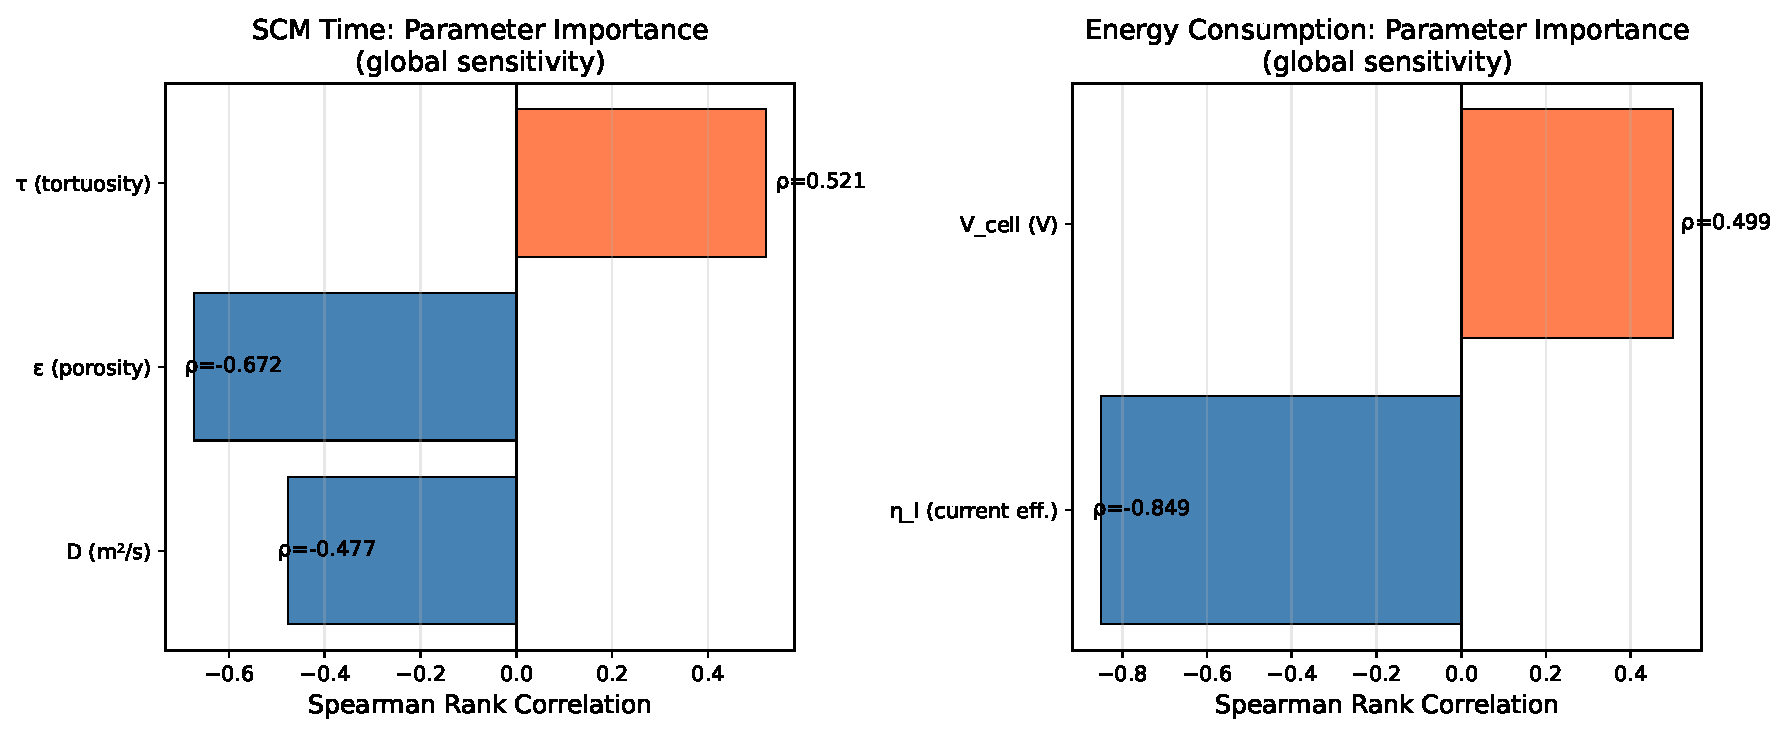
\includegraphics[width=0.95\linewidth]{fig_sensitivity_tornado.pdf}
\caption{Global parameter sensitivity (Spearman rank correlation): (left) SCM reduction time; (right) net energy consumption.}
\label{fig:tornado}
\end{figure}

\begin{figure}[!ht]
\centering
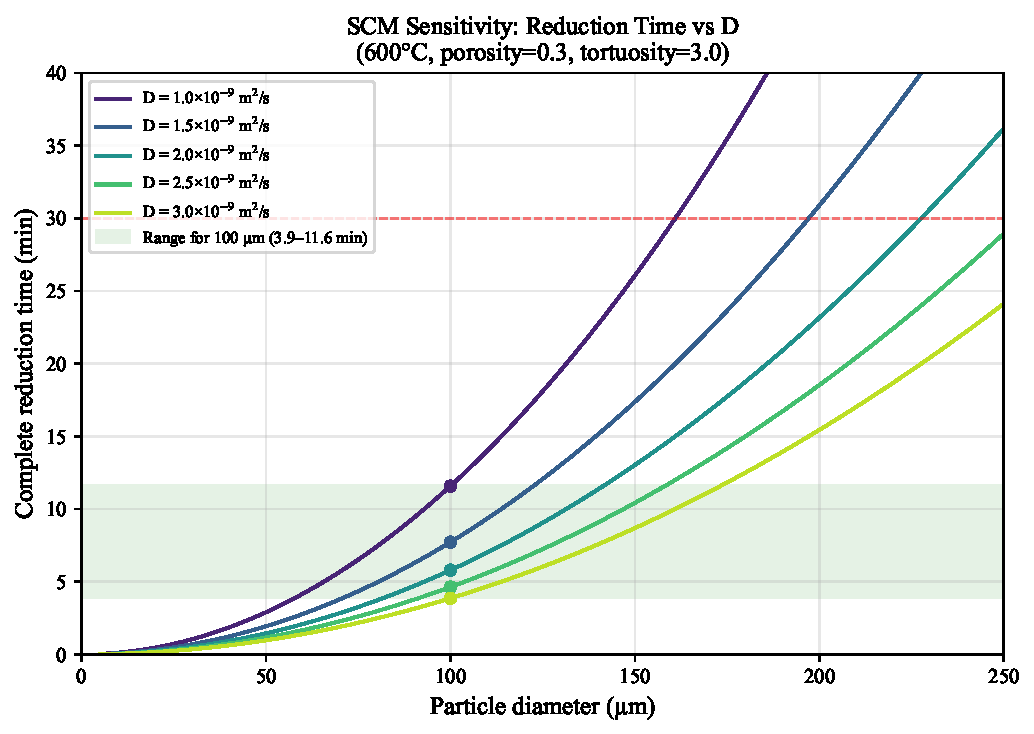
\includegraphics[width=0.95\linewidth]{fig_scm_sensitivity.pdf}
\caption{SCM sensitivity analysis: reduction time versus particle diameter for $D = 1$--$3\times10^{-9}$~m$^2$/s.}
\label{fig:scm_sens}
\end{figure}

\begin{figure}[!ht]
\centering
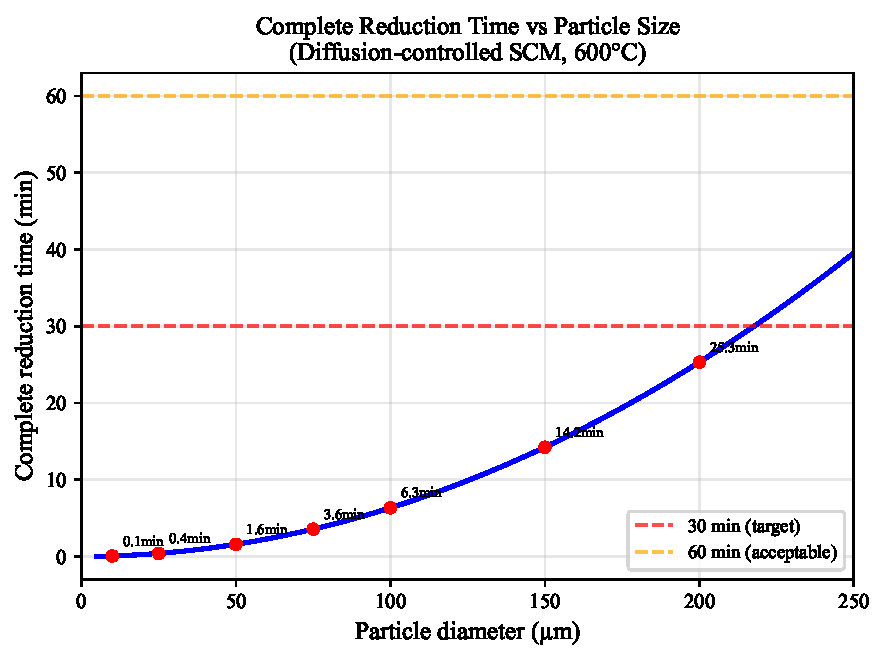
\includegraphics[width=0.95\linewidth]{fig_scm_time_vs_size.pdf}
\caption{Complete reduction time versus particle diameter at $D = 2.0\times10^{-9}$~m$^2$/s (600~$^{\circ}$C), showing the inverse-square scaling.}
\label{fig:scm_time}
\end{figure}

\subsection{Material and Energy Balance}
\label{subsec:energy}

The material balance per ton Ti is split into two steps: (i) the chemical reduction step and (ii) the electrolytic regeneration step. In Step~(i), $\ce{TiO2}$ is reduced by Mg and Ca:
\begin{equation}
\ce{TiO2 + Mg + Ca -> Ti + MgO + CaO} \quad (3013~\mathrm{kg} = 3013~\mathrm{kg})
\end{equation}
In Step~(ii), the by-product oxides are electrolytically regenerated:
\begin{equation}
\ce{MgO + CaO -> Mg + Ca + O2} \quad (2013~\mathrm{kg} = 2013~\mathrm{kg})
\end{equation}
The net reaction is $\ce{TiO2 -> Ti + O2}$ ($1668~\mathrm{kg} = 1668~\mathrm{kg}$), with Mg and Ca acting as cyclic mediators. When using 90~wt\% metallurgical-grade $\ce{TiO2}$ ore, the impurity mass (186~kg/ton-Ti, mainly $\ce{Fe2O3}$ and $\ce{SiO2}$) enters as part of the ore input and exits as reduced impurity metals (Fe, Si), which require separation from the Ti product as discussed in Section~4.3.

\begin{table}[!ht]
\centering
\footnotesize
\caption{Material balance (basis: 1 ton Ti, pure $\ce{TiO2}$)}
\label{tab:mbalance}
\begin{tabular}{llc}
\toprule
Category & Item & Mass (kg) \\
\midrule
Input & $\ce{TiO2}$ (pure) & 1668 \\
 & Mg (cyclic) & 508 \\
 & Ca (cyclic) & 837 \\
\midrule
Output & Ti metal & 1000 \\
 & $\ce{MgO}$ (to regeneration) & 842 \\
 & $\ce{CaO}$ (to regeneration) & 1171 \\
\midrule
Check & Input total & 3013 \\
 & Output total & 3013 \\
\midrule
Net & $\ce{TiO2} \to \ce{Ti} + \ce{O2}$ & 1668 = 1000 + 668 \\
\bottomrule
\end{tabular}
\end{table}

The theoretical decomposition voltage for simultaneous regeneration of MgO and CaO (4~e$^-$ per mol Ti) is 2.73~V, giving a theoretical minimum electrolysis energy of 6112~kWh/ton-Ti. The assumed cell voltage ($\sim$4.1~V) is decomposed as $V_{\mathrm{cell}} = E_{\mathrm{decomp}} + \eta_{\mathrm{anode}} + \eta_{\mathrm{cathode}} + IR_{\mathrm{ohm}}$ (Fig.~\ref{fig:voltage_split}): the 2.73~V decomposition term is augmented by $\sim$0.30~V anode overpotential ($\ce{O2}$ evolution), $\sim$0.20~V cathode overpotential (Mg/Ca deposition), and $\sim$0.90~V ohmic drop (melt conductivity, contacts, busbars), summing to $\sim$4.13~V. These overpotential and ohmic terms are order-of-magnitude estimates, but they make explicit where the voltage---and hence the energy---is spent, and identify the anode overpotential and ohmic drop as the primary targets for cell design. Practical energy consumption depends on current efficiency $\eta_I$ and cell voltage $V_{\mathrm{cell}}$:
\begin{equation}
W_{\mathrm{practical}} = \frac{4F \cdot n_{\mathrm{Ti}} \cdot V_{\mathrm{cell}}}{\eta_I \cdot 3.6\times10^{6}}
\end{equation}

\begin{table}[!ht]
\centering
\footnotesize
\caption{Practical energy consumption (basis: 1 ton Ti)}
\label{tab:energy}
\begin{tabular}{cccl}
\toprule
$\eta_I$ & $V_{\mathrm{cell}}$ (V) & Energy (kWh/ton) & Condition \\
\midrule
0.85 & 3.5 & 9222 & Best \\
0.80 & 4.0 & 11198 & Moderate \\
0.75 & 4.0 & 11944 & Conservative \\
0.75 & 4.3 & 12840 & Graphite anode + ohmic \\
0.70 & 4.5 & 14397 & Worst \\
\bottomrule
\end{tabular}
\end{table}

\begin{figure}[!ht]
\centering
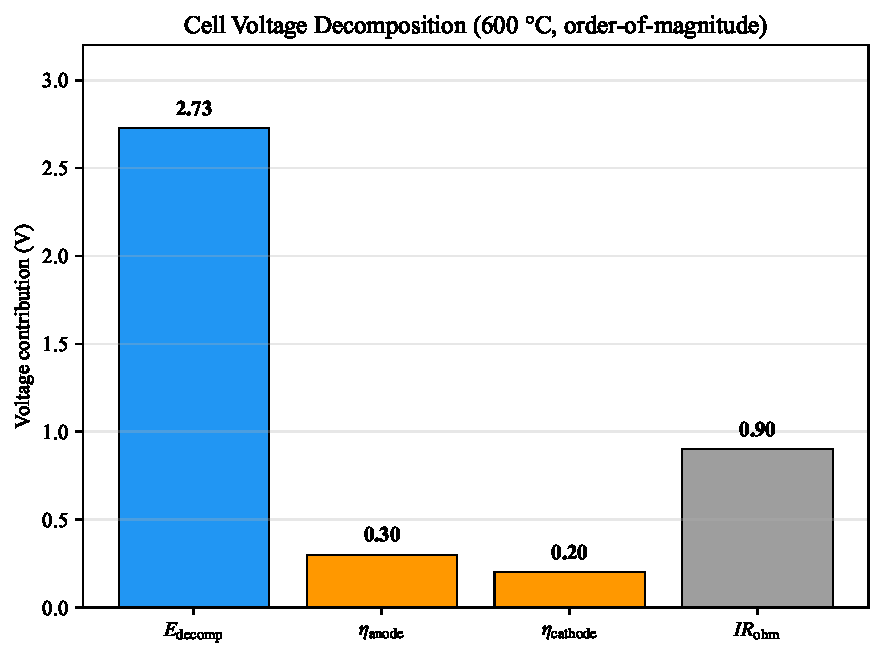
\includegraphics[width=0.7\linewidth]{fig_voltage_split.pdf}
\caption{Decomposition of the assumed cell voltage ($\sim$4.1~V) into the thermodynamic decomposition term (2.73~V), anode and cathode overpotentials, and ohmic drop (order-of-magnitude estimates).}
\label{fig:voltage_split}
\end{figure}

Under realistic conditions ($\eta_I = 0.75$--0.80, $V_{\mathrm{cell}} = 4.0$--4.3~V), the electrolysis-step energy consumption is 11{,}200--12{,}800~kWh/ton-Ti (electrolysis step only; full-process net consumption is 11{,}192~kWh/ton-Ti, see Sec.~\ref{subsec:heatbal}). The sensitivity analysis (Fig.~\ref{fig:energy}) shows that $\eta_I \geq 74.7\%$ at $V = 4.0$~V is required to stay below 12{,}000~kWh/ton.

The assumed current efficiency range ($\eta_I = 0.75$--0.80) requires justification, as it significantly exceeds the FFC Cambridge process (30--50\%) \cite{fray2000}. The key difference is that FFC involves direct electro-deoxidation of solid $\ce{TiO2}$ at the cathode, where slow solid-state diffusion and side reactions cause severe current leakage. In the proposed process, electrolysis targets dissolved MgO and CaO rather than a solid oxide cathode. This mechanism bears greater mechanistic similarity to the Hall--H\'eroult process, where dissolved $\ce{Al2O3}$ is electrolyzed with current efficiencies of 90--95\% under industrial conditions \cite{kvande2014}. Although the higher decomposition voltage and the chemical reactivity of Mg/Ca may introduce additional loss pathways absent in aluminum electrolysis, the dissolved-oxide route fundamentally avoids solid-state diffusion limitations, providing a mechanistic basis for expecting current efficiencies substantially higher than those of the FFC process. The target range of 75--80\% is therefore an \emph{unvalidated hypothesis} rather than a physically established result. This is further supported by the Downs process for sodium production (70--90\%) and by industrial Mg electrolysis from molten $\ce{MgCl2}$---the primary salt of the present process---which achieves 80--90\% current efficiency, both well-established for dissolved-salt electrolysis in chloride melts \cite{plettcher1990,ji2026}. The main current efficiency loss mechanisms expected in this process are: (i) electronic conduction through the melt, estimated at 2--5\% loss; (ii) back-reaction between deposited Mg/Ca and dissolved O$^{2-}$ at the anode--cathode interface, estimated at 5--10\% loss depending on cell geometry; (iii) Na co-deposition at high current densities, estimated at 3--8\% loss; and (iv) impurity-related side reactions, estimated at 2--5\% loss. Summing these estimates yields $\eta_I \approx 0.72$--0.88, centered on the assumed 0.75--0.80 range. The loss mechanisms are assumed additive and independent; potential overlap (e.g., between electronic conduction and parasitic reactions) is not quantified. However, it must be emphasized that these estimates are preliminary. The analogy to Hall--H\'eroult and Downs processes provides an upper-bound estimate; the actual $\eta_I$ in a TiO$_2$ reduction system may differ due to side reactions specific to this chemistry, such as formation of sub-valent titanium chlorides (TiCl$_2$, TiCl$_3$) that consume current without producing useful reductant, and re-oxidation of deposited Mg/Ca by dissolved O$^{2-}$ at higher rates than in Al or Na systems due to the higher chemical reactivity of Mg and Ca. If $\eta_I$ proves to be only 0.50--0.60 (comparable to FFC), the energy consumption would rise to 14{,}000--19{,}000~kWh/ton-Ti, approaching the FFC range (15{,}000--20{,}000~kWh/ton-Ti). Therefore, the ``energy-efficient'' characterization of this process is \emph{conditional on achieving $\eta_I > 0.70$}.

For context, the Kroll process consumes approximately 30{,}000--40{,}000~kWh/ton-Ti (industrial measured, including chlorination, Mg reduction, and vacuum distillation) \cite{ji2026}, while the FFC Cambridge process is estimated at 15{,}000--20{,}000~kWh/ton-Ti (pilot-scale measured, due to lower current efficiency of 30--50\% and higher operating temperature of $\sim$950~$^{\circ}$C) \cite{fray2000,ji2026}. The proposed process predicts 11{,}200--12{,}800~kWh/ton-Ti (\emph{theoretical prediction} based on assumed $\eta_I = 0.75$--0.80 and $V_{\mathrm{cell}} = 4.0$--4.3~V) primarily through reduced operating temperature (600~$^{\circ}$C), higher target current efficiency (75--80\%, conditional on achieving dissolved-oxide electrolysis performance comparable to Hall--H\'eroult and Downs processes), and elimination of the chlorination step. It should be emphasized that these are \emph{non-equivalent comparisons}: the proposed process values are theoretical predictions based on assumed parameters, while the Kroll and FFC figures are industrial/pilot-scale measured values with different system boundaries. A rigorous comparison requires unified cradle-to-gate boundary analysis.

A particularly relevant analogy is the Hall--H\'eroult process for aluminum production \cite{kvande2014}, which also electrolyzes a dissolved oxide ($\ce{Al2O3}$ in cryolite melt) rather than a solid cathode. Hall--H\'eroult achieves current efficiencies of 90--95\% at $\sim$950~$^{\circ}$C with DC energy consumption of $\sim$13{,}000~kWh/ton-Al and cell voltages of 4.0--4.2~V. The proposed Ti process shares the dissolved-oxide electrolysis mechanism but operates at significantly lower temperature (600~$^{\circ}$C), which reduces thermal losses and material corrosion. However, the higher decomposition voltage of $\ce{TiO2}$ (thermodynamic minimum $\sim$2.73~V vs.\ $\sim$1.18~V for $\ce{Al2O3}$) and the additional overpotentials for Mg/Ca co-deposition result in a higher cell voltage ($\sim$4.0--4.3~V). If the dissolved-oxide electrolysis mechanism can be confirmed experimentally, the Hall--H\'eroult analogy supports the feasibility of achieving $\eta_I > 0.70$, since the fundamental current-loss mechanisms (electronic conduction, back-reaction) are mitigated by the lower operating temperature and the chemical mediation via Mg/Ca cycling.

\begin{figure}[!ht]
\centering
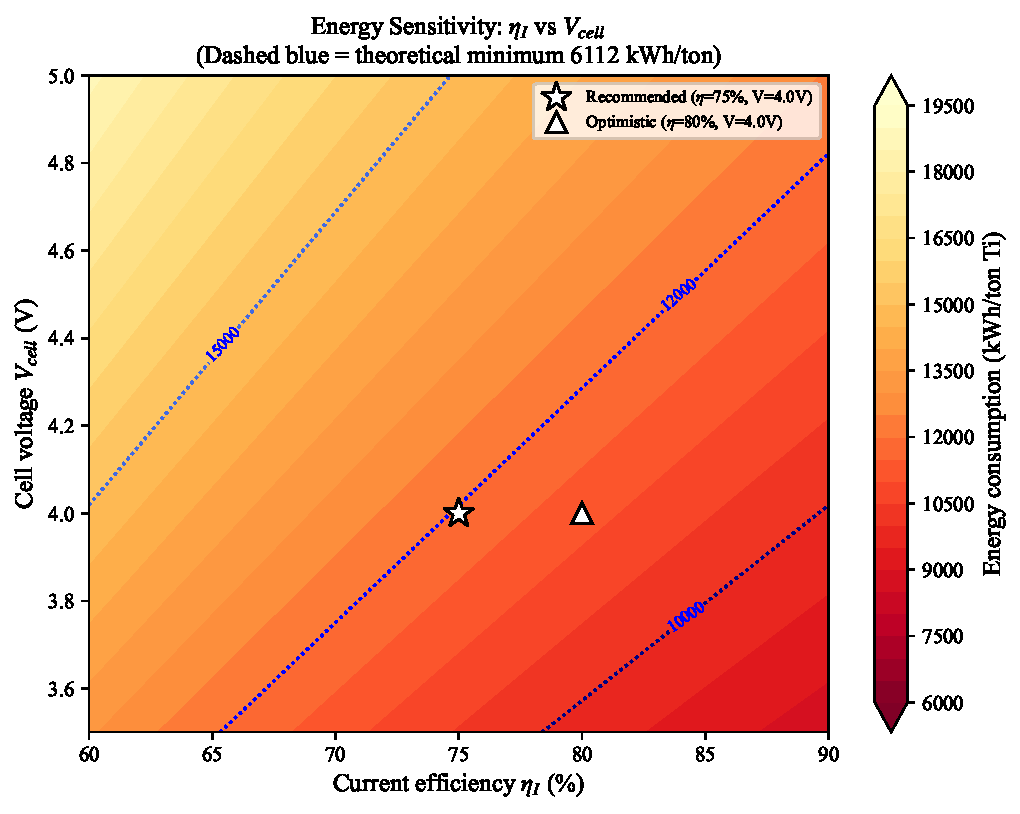
\includegraphics[width=0.95\linewidth]{fig_energy_sensitivity.pdf}
\caption{Energy sensitivity: $\eta_I$ vs.\ $V_{\mathrm{cell}}$ (practical range; the electrolysis step minimum 6112~kWh/ton and the net reaction reversible work $\sim$4550~kWh/ton both lie below this range and are not shown).}
\label{fig:energy}
\end{figure}

\subsection{Full-Process Energy Balance}
\label{subsec:heatbal}

The full-process energy balance (Table~\ref{tab:heatbal}), \emph{conditional on achieving $\eta_I > 0.70$} as discussed in Sec.~\ref{subsec:energy}, is structured to distinguish electrical energy inputs from thermal effects. The electrolysis gross electrical demand is 12{,}244~kWh/ton ($\eta_I=0.75$, $V_{\mathrm{cell}}=4.1$~V). The exothermic reduction reaction releases 1{,}690~kWh/ton of thermal energy, which is treated as an equivalent internal heat source that reduces the equivalent external energy requirement; this yields a net equivalent electrolysis input of 10{,}554~kWh/ton. Auxiliary processes (preheating, pumping, post-treatment) contribute 680~kWh/ton, giving a total equivalent external input of 11{,}234~kWh/ton. Ti powder cooling recovers 42~kWh/ton, yielding a net equivalent consumption of 11{,}192~kWh/ton-Ti.

\emph{It is important to note that the treatment of the reaction exotherm as an offset to the gross electrical demand is a simplified accounting convention. Strictly, thermal energy and electrical energy are distinct in quality (exergy): reaction heat (chemical energy converted to thermal energy) cannot directly substitute for electrical energy at 100\% conversion efficiency. The 11{,}192~kWh/ton figure therefore represents an \emph{equivalent net external energy demand} rather than a rigorous thermodynamic minimum. A separate exergetic analysis---which accounts for the Carnot-limited convertibility of heat to work---would yield a higher effective energy consumption: crediting the 1{,}690~kWh/ton exotherm at its Carnot work-equivalent (factor $1 - 298/873 \approx 0.66$, i.e., $\sim$1{,}100~kWh/ton) instead of 1:1 would raise the net equivalent consumption to $\sim$11{,}800~kWh/ton.} The process energy efficiency, defined here as the ratio of the electrolysis step's theoretical minimum (6{,}112~kWh/ton) to the net equivalent external energy consumption (11{,}192~kWh/ton), is 54.6\% ($= 6112/11192$), reflecting the combined irreversibilities of electrolysis (voltage efficiency $\sim$68\%, current efficiency 75--80\%) and thermal losses. It is important to distinguish this from the true second-law (exergetic) efficiency: the net reaction $\ce{TiO2 -> Ti + O2}$ has a reversible work of $\sim$4{,}550~kWh/ton-Ti ($\Delta G^{\circ}_{\ce{TiO2}} \approx 783$~kJ/mol at 873~K), yielding a second-law efficiency of $\sim$40.7\% ($= 4550/11192$). In summary, the 54.6\% figure represents the ratio of the electrolysis step's theoretical minimum ($\ce{MgO + CaO -> Mg + Ca + O2}$, 6{,}112~kWh/ton) to the equivalent net energy consumption, whereas the 40.7\% figure represents the ratio of the overall reaction's reversible Gibbs free energy ($\ce{TiO2 -> Ti + O2}$, 4{,}550~kWh/ton) to the same denominator; the difference arises because the electrolysis step minimum exceeds the net reaction reversible work due to the additional energy required for Mg/Ca regeneration. The electrolysis energy fraction of 93.9\% ($= 10554/11234$) indicates that electrolysis dominates the energy budget; it is \emph{not} a thermodynamic efficiency. Regarding the heat balance, the reaction exotherm (1{,}690~kWh/ton) is \emph{accounted for} as an equivalent offset to the gross demand (12{,}244 $\to$ 10{,}554~kWh/ton) in the simplified energy accounting and is \emph{not} additionally applied to the cell wall heat loss (138~kWh/ton), which is a separate external thermal requirement supplied by auxiliary heating.

\begin{table}[!ht]
\centering
\footnotesize
\caption{Full-process heat balance (basis: 1 ton Ti, 600~$^{\circ}$C)}
\label{tab:heatbal}
\begin{tabularx}{\linewidth}{l c X}
\toprule
Item & Energy (kWh/ton) & Note \\
\midrule
\multicolumn{3}{l}{\textit{Electrolysis}} \\
\quad Gross electrical demand & 12244 & $W = 4F n_{\mathrm{Ti}} V_{\mathrm{cell}}/(\eta_I \cdot 3.6{\times}10^6)$ at $\eta_I=0.75$, $V_{\mathrm{cell}}=4.1$~V \\
\quad Reaction exotherm (equiv.~offset) & $-$1690 & From $\Delta H^{\circ}_{\mathrm{R1{+}R2}} \approx -291.3$~kJ/mol-Ti$^{\mathrm{a}}$ \\
\quad Net equivalent electrolysis input & 10554 & Equiv.~external energy demand \\
\midrule
\multicolumn{3}{l}{\textit{Auxiliary inputs}} \\
\quad $\ce{TiO2}$ preheating & 184 & External thermal input \\
\quad Salt makeup preheating & 8 & External thermal input \\
\quad Cell wall heat loss & 138 & External thermal input \\
\quad Salt circulation pumping & 50 & External input \\
\quad Post-treatment (washing/drying/screening) & 300 & External input (excludes impurity acid-leaching, see Limitations~(7)) \\
\midrule
\quad Total external input & 11234 & \\
\midrule
\multicolumn{3}{l}{\textit{Heat recovery}} \\
\quad Ti powder cooling (50\% recoverable) & 42 & External heat recovery \\
\midrule
\multicolumn{3}{l}{\textit{Net consumption}} \\
\quad Net energy & 11192 & Total input $-$ Ti cooling \\
\quad Electrolysis step minimum & 6{,}112 & $\ce{MgO + CaO -> Mg + Ca + O2}$ at 873~K \\
\quad Net reaction reversible work & $\sim$4{,}550 & $\ce{TiO2 -> Ti + O2}$, $\Delta G^{\circ}\approx783$~kJ/mol at 873~K \\
\quad Process energy efficiency & 54.6\% & $6112/11192$ (equiv.) \\
\quad Second-law efficiency & $\sim$40.7\% & $4550/11192$ \\
\quad Electrolysis energy fraction & --- & 93.9\% ($W_{\mathrm{elec}}/W_{\mathrm{total}}$) \\
\bottomrule
\end{tabularx}

\par\footnotesize $^{\mathrm{a}}$\,Simplified accounting: the reaction exotherm ($\Delta H^{\circ} = -291.3$~kJ/mol-Ti for the combined Mg+Ca reduction, from Table~\ref{tab:thermo}; $291.3 \times 20889 / 3600 \approx 1690$~kWh/ton-Ti) is treated as an equivalent offset to the gross electrical demand. Strictly, thermal and electrical energy differ in exergy; see Sec.~\ref{subsec:heatbal} text.
\end{table}

For comparison, the minimum thermodynamic work for $\ce{TiCl4}$ distillation (90\% $\to$ 99.9\%, 99\% recovery) in the Kroll process is 5.7~kWh/ton-Ti (estimated from the ideal-solution minimum work of separation at 136~$^{\circ}$C, $\Delta G_{\mathrm{sep}} = RT \sum_k n_k \sum_i x_{i,k}\ln(x_{i,k}/x_{i,\mathrm{feed}})$ summed over the product and waste streams $k$ and components $i = \{\ce{TiCl4}, \mathrm{impurity}\}$), while the actual distillation consumes $\sim$300~kWh/ton-Ti---a second-law efficiency of 1.9\% ($= 5.7/300$). The proposed process eliminates this separation step entirely by using metallurgical-grade $\ce{TiO2}$ directly.

\subsection{Oxide Dissolution Mechanism and Salt Circulation}
\label{subsec:dissolution}

A critical feature of the process is the dissolution of $\ce{MgO}$ and $\ce{CaO}$ in the $\ce{CaCl2}$-containing melt. Ito and Morita \cite{morita2004} measured $\ce{MgO}$ solubility of 2.35~wt\% in $\ce{MgCl2-CaCl2}$ melt at 800~$^{\circ}$C, with solubility increasing significantly with $\ce{CaCl2}$ content. It should be noted that the actual operating temperature (580--650~$^{\circ}$C) is 150--250~$^{\circ}$C lower than the measurement temperature, and oxide solubility typically decreases with temperature. A rough Arrhenius extrapolation suggests that the solubility at 600~$^{\circ}$C may be approximately 0.5--1.2~wt\% (roughly 30--50\% of the 800~$^{\circ}$C value), which still provides meaningful dissolution capacity but at a reduced rate. This estimate is an \emph{order-of-magnitude estimate based on single-point Arrhenius extrapolation}: due to the lack of multi-temperature solubility data, the activation energy $E_a$ is not independently determined, and the estimated range carries a factor-of-2.4 uncertainty. The extrapolation parameters (activation energy, number of data points, and confidence interval) are not available in the literature; the estimate is based on the general trend that oxide solubility in chloride melts decreases with temperature following an Arrhenius relationship. Within the estimated 0.5--1.2~wt\% range, the reduced solubility would increase the required salt circulation rate by a factor of 2--4 compared to the 800~$^{\circ}$C baseline, which is theoretically manageable. To fix the scale: at 1~wt\% oxide solubility the salt inventory needed to hold the 2013~kg of MgO+CaO produced per ton Ti is $\sim$201~t of salt per ton Ti (117~t for CaO alone and 84~t for MgO), rising to $\sim$400~t at 0.5~wt\%. This is a large but not unphysical inventory---comparable to the cryolite inventory of industrial Hall--H\'eroult cells---and the \emph{circulation rate} (t/h) is set by the production rate rather than by this inventory. However, if the actual 600~$^{\circ}$C solubility falls below 0.5~wt\%, the required salt inventory and circulation rate increase by more than 4$\times$, potentially invalidating the closed-loop design. \textbf{The closed-loop salt circulation is therefore a theoretical hypothesis pending experimental validation of 600~$^{\circ}$C oxide solubility---this is the most critical experimental uncertainty in the present process concept.} The dissolution mechanism involves the formation of calcium oxychloride complexes:
\begin{align}
\ce{CaO(s) &-> Ca^{2+} + O^{2-}} \label{eq:diss1} \\
\ce{O^{2-} + 2Ca^{2+} &-> [Ca2O]^{2+}} \label{eq:diss2} \\
\ce{O^{2-} + 3Ca^{2+} &-> [Ca3O]^{4+}} \label{eq:diss3}
\end{align}
The association of $\ce{O^{2-}}$ with $\ce{Ca^{2+}}$ reduces the free oxygen ion activity, driving further oxide dissolution. This mechanism explains why $\ce{CaCl2}$-rich melts exhibit higher oxide solubility: the $\ce{Ca^{2+}}$ ions act as solvation agents for $\ce{O^{2-}}$, lowering its effective activity and shifting the dissolution equilibrium forward. Quantitative modeling of these equilibria requires complexation constants that are not well-established in the open literature; however, the qualitative mechanism is consistent with both the solubility data of Ito and Morita \cite{morita2004} and the MQM framework of the FactSage Salt database \cite{pelton2000mqm}, which explicitly models short-range ordering in charge-unsymmetrical chloride melts through pair exchange reactions.

The reduced free $\ce{O^{2-}}$ activity also affects the anode potential for oxygen evolution. For the anode half-reaction $\ce{2O^{2-} -> O2 + 4e^-}$, the Nernst equation (assuming $p_{\ce{O2}} = 1$~atm) gives the reduction-direction electrode potential:
\begin{equation}
\label{eq:anode}
E_{\mathrm{anode}} = E^{\circ}_{\ce{O2/O^{2-}}} - \frac{RT}{4F}\ln(a_{\ce{O^{2-}}}^2) = E^{\circ}_{\ce{O2/O^{2-}}} - \frac{RT}{2F}\ln(a_{\ce{O^{2-}}})
\end{equation}
Lower $a_{\ce{O^{2-}}}$ (due to complexation) shifts the anode potential positively (since $-\ln(a_{\ce{O^{2-}}})$ increases as $a_{\ce{O^{2-}}}$ decreases), meaning a higher applied voltage is required for oxygen evolution. This narrows the selectivity window between $\ce{O2}$ and $\ce{Cl2}$ evolution, necessitating careful anode potential control in the $\ce{CaCl2}$-containing system.

\textbf{Anode-selectivity boundary condition.} The competing chloride oxidation $\ce{2Cl^- -> Cl2 + 2e^-}$ sits at $E_{\mathrm{red}}(\ce{Cl2/Cl^-}) = 0$ by the reference convention of Table~\ref{tab:Ed} (with $a_{\ce{Cl^-}} \approx 1$). Oxygen evolution is thermodynamically favored only while $E_{\mathrm{red}}(\ce{O2/O^{2-}}) < 0$; from Eq.~\ref{eq:anode} this requires
\begin{equation}
E^{\circ}_{\ce{O2/O^{2-}}}(\mathrm{vs}~\ce{Cl2/Cl^-}) \;<\; \frac{RT}{2F}\ln(a_{\ce{O^{2-}}}),
\end{equation}
i.e., the free oxide-ion activity must stay above the threshold $a_{\ce{O^{2-}}} > \exp\!\big[2F\,E^{\circ}_{\ce{O2/O^{2-}}}(\mathrm{vs}~\ce{Cl2/Cl^-})/(RT)\big]$, otherwise $\ce{Cl2}$ evolution is thermodynamically preferred. The standard potential $E^{\circ}_{\ce{O2/O^{2-}}}(\mathrm{vs}~\ce{Cl2/Cl^-})$ is the melt's \emph{oxoacidity} (the standard free energy of $\ce{O^{2-} + Cl2 -> 1/2\,O2 + 2Cl^-}$), a melt-specific quantity that has not been reported for the quaternary $\ce{MgCl2-CaCl2-NaCl-KCl}$ system and cannot be inferred from pure oxide/chloride formation data alone. Until this oxoacidity is measured or obtained from a CALPHAD salt-model (MQM) calculation, the critical $a_{\ce{O^{2-}}}$ below which $\ce{Cl2}$ evolution becomes competitive is a missing quantitative boundary for the closed-loop $\ce{O2}$-evolution assumption underlying the energy balance.

Fig.~\ref{fig:cl2} renders this boundary parametrically: the critical free oxide activity $a_{\ce{O^{2-}},crit} = \exp[2F\,E^{\circ}(\mathrm{vs}~\ce{Cl2/Cl^-})/(RT)]$ is plotted against the oxoacidity $E^{\circ}$. The actual free-oxide activity in the melt is estimated from the oxide solubility (Sec.~\ref{subsec:dissolution}): $\sim$1~wt\% dissolved oxide corresponds to a formal $x_{\ce{O^{2-}}} \sim 10^{-2}$, and the strong $\ce{Ca^{2+}}$--$\ce{O^{2-}}$ complexation reduces the \emph{free} $a_{\ce{O^{2-}}}$ by roughly 1--2 orders of magnitude, placing the operating point in the range $a_{\ce{O^{2-}}} \approx 10^{-4}$--$10^{-3}$. Oxygen evolution is therefore safe (the operating point lies above the critical line) only if the oxoacidity is more negative than $\approx -0.35$~V; conversely, if $E^{\circ}(\mathrm{vs}~\ce{Cl2/Cl^-})$ is less negative than $\approx -0.26$~V, the operating point falls below the critical line and $\ce{Cl2}$ evolution becomes thermodynamically preferred. These two thresholds are \emph{not} measured oxoacidities: they follow from substituting the assumed operating bounds ($a_{\ce{O^{2-}}} = 10^{-4}$ and $10^{-3}$) back into $a_{\ce{O^{2-}},crit}$, so they serve only to locate the boundary relative to the estimated operating band. Because typical chloride-melt oxoacidities span roughly this range, the anode selectivity cannot be assumed \emph{a priori} and must be established for the specific quaternary composition. This coupling between oxide dissolution and electrochemistry is a distinctive feature of the $\ce{CaCl2}$-containing system.

\begin{figure}[!ht]
\centering
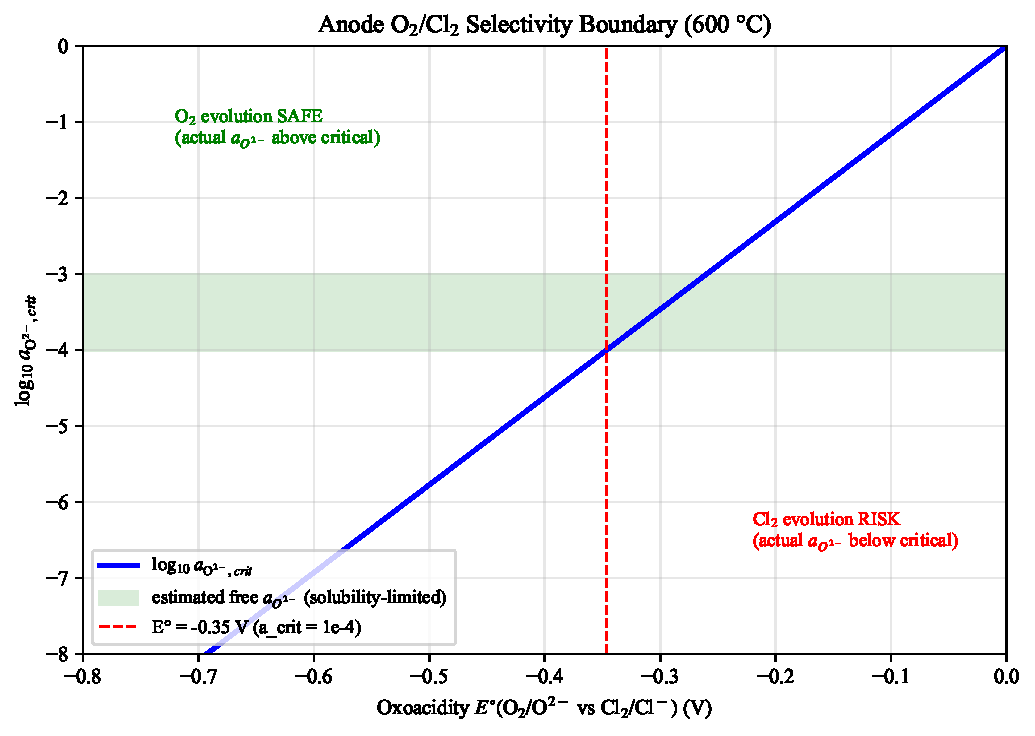
\includegraphics[width=0.85\linewidth]{fig_cl2_boundary.pdf}
\caption{Anode $\ce{O2}$/$\ce{Cl2}$ selectivity boundary at 600~$^{\circ}$C. The critical free-oxide activity $a_{\ce{O^{2-}},crit}$ (solid line) is plotted as a function of the melt oxoacidity $E^{\circ}(\ce{O2/O^{2-}}~\text{vs}~\ce{Cl2/Cl^-})$, which has not been measured for this quaternary system. The green band is the estimated operating $a_{\ce{O^{2-}}}$ from oxide solubility and $\ce{Ca^{2+}}$--$\ce{O^{2-}}$ complexation. The marked crossing ($E^{\circ} \approx -0.35$~V) is derived from the assumed $a_{\ce{O^{2-}}}$ range ($10^{-4}$--$10^{-3}$), not from any measured oxoacidity; $\ce{O2}$ evolution is thermodynamically favored only to its left.}
\label{fig:cl2}
\end{figure}

A second, coupled consequence of anode-side $\ce{Cl2}$ evolution is the chemical attack of the Ti product by dissolved chlorine. Molten-salt titanium electrochemistry is well known to suffer a ``valence cycle'' current-efficiency loss in which Ti metal reacts with $\ce{Cl2}$/$\ce{TiCl4}$ to form the soluble lower chlorides $\ce{TiCl2}$/$\ce{TiCl3}$, which are then re-oxidized at the anode, shuttling charge without net Ti production. In the present process this cycle is suppressed \emph{only} while the anode remains selective to $\ce{O2}$ (Fig.~\ref{fig:cl2}): any drift into the $\ce{Cl2}$-evolution regime not only degrades the closed-loop $\ce{O2}$ assumption but also re-introduces the dominant current-loss mechanism of chloride-based titanium electrochemistry. This further underscores that the oxoacidity---and hence the $\ce{O2}$/$\ce{Cl2}$ anode selectivity---is the pivotal missing measurement for the proposed process, on a par with the 600~$^{\circ}$C oxide solubility.

The thermodynamic driving force of this cycle is substantial (Table~\ref{tab:ticl}): all three titanium chlorides are strongly stable relative to the elements, and the disproportionation $\ce{Ti + TiCl4 -> 2TiCl2}$ has $\Delta G^{\circ}(298~\mathrm{K}) \approx -202$~kJ/mol, remaining exergonic ($\approx -80$~kJ/mol) at 873~K when estimated from the 298~K enthalpy/entropy of formation. Thus, whenever free $\ce{Cl2}$ or $\ce{TiCl4}$ is present, the Ti cathode product is thermodynamically unstable against dissolution as $\ce{TiCl2}$/$\ce{TiCl3}$, which then migrate to the anode and are re-oxidized---the classic current-efficiency killer of chloride-based Ti electrolysis. The proposed process suppresses this only by keeping the anode in the $\ce{O2}$ regime of Fig.~\ref{fig:cl2}.

\begin{table}[!ht]
\centering
\footnotesize
\caption{Standard Gibbs free energies of formation of titanium chlorides (Barin \cite{barin1995}, 298~K, approximate) and the $\ce{Ti + TiCl4 -> 2TiCl2}$ disproportionation.}
\label{tab:ticl}
\begin{tabular}{lc}
\toprule
Species / reaction & $\Delta G^{\circ}$ (kJ/mol) \\
\midrule
$\ce{TiCl2(s)}$ & $-464$ \\
$\ce{TiCl3(s)}$ & $-654$ \\
$\ce{TiCl4(g)}$ & $-727$ \\
$\ce{Ti + TiCl4 -> 2TiCl2}$ (298~K) & $-202$ \\
$\ce{Ti + TiCl4 -> 2TiCl2}$ (873~K, est.) & $\approx -80$ \\
\bottomrule
\end{tabular}

\par\footnotesize The 873~K value is estimated as $\Delta G(873) \approx \Delta H^{\circ}(298) - 873\,\Delta S^{\circ}(298)$ using the 298~K Barin enthalpy and entropy of formation (neglecting $C_p$ temperature dependence).
\end{table}

\section{Process Comparison}

Table~\ref{tab:compare} compares the proposed process with established technologies. The key distinction is the electrochemical-thermochemical coupling: unlike FFC (pure electro-deoxidation) or Kroll (pure metallothermic), this process uses electrolysis to regenerate reductants in situ while leveraging bimetallic complementary reduction for both rate and purity.

\begin{table}[!ht]
  \centering
  \caption{Comparison of titanium production processes}
  \label{tab:compare}
  \footnotesize
  \begin{tabularx}{\linewidth}{@{} p{1.5cm} p{3.0cm} p{1.2cm} p{1.0cm} p{1.2cm} p{1.0cm} X @{}}
  \toprule
  Process & Core Principle & Mode & Temp. ($^{\circ}$C) & Energy & Purity & Key Challenge \\
  \midrule
  Kroll & Chlorination + Mg reduction & Batch & 1000--1200 & Very high & High & Long process, pollution \\
  FFC & Direct electro-deoxidation & Batch & $\sim$950 & High & Moderate & Low current efficiency \\
  OS & Electrolytic Ca regeneration + calciothermic reduction & Cyclic & $\sim$900 & High & High & Ca reactivity, high temp. \\
  SOM & Solid oxide membrane electrolysis & Semi-cont. & 700--800 & Moderate & High & Membrane durability \\
  USTB & Anode dissolution-deposition & Semi-cont. & $\sim$900 & High & High & Anode loss \\
  Proposed & In-situ electrolysis + Mg-Ca complementary reduction & Cyclic (conceptual) & 580--650 & Moderate$^{a}$ & High (target) & Anode corrosion, unvalidated $\eta_I$ \\
  \bottomrule
  \end{tabularx}
  \par\vspace{2pt}
  \footnotesize $^{a}$Theoretical prediction conditional on $\eta_I > 0.70$; industrial/pilot values shown for Kroll/FFC/USTB are not directly equivalent.
\end{table}

\section{Uncertainties and Limitations}

This study is a conceptual design based on thermodynamic calculations and literature data. All quantitative results require future experimental validation; the key uncertainties are acknowledged below:

(1) \textbf{Activity coefficients}: The ideal solution assumption introduces uncertainty in the co-deposition window; the sensitivity analysis (Section~\ref{subsec:activity}) suggests viability for $\gamma_{\ce{CaCl2}} = 0.3$--1.0, but precise values require FactSage/MQM calculation or direct measurement.

(2) \textbf{Electrode overpotentials and Mg/Ca co-deposition ratio}: The co-deposition window analysis is based on equilibrium Nernst equations. In practice, activation overpotentials (Butler--Volmer), concentration polarization, and ohmic drops modify the effective window. Qualitative analysis suggests that Na$^+$ may exhibit a higher activation overpotential than Ca$^{2+}$, which may \emph{enlarge} the practical window; however, the sign of this kinetic correction is not established---the Downs cell deposits Na from a $\ce{CaCl2}$-majority melt, suggesting $\ce{Ca^{2+}}$ reduction may instead be kinetically slower, which would \emph{narrow} the window. Quantitative assessment therefore requires electrode-kinetic parameters (exchange current density, transfer coefficient) that are not currently available for the quaternary chloride melt. A further and larger uncertainty is the Mg/Ca co-deposition ratio: because Mg reduces $\sim$816~mV earlier than Ca, the equimolar Mg--Ca alloy assumed in the material balance and Sec.~\ref{subsec:MgCa} can only be approached when Mg deposition reaches its mass-transfer (diffusion) limit, and the actual ratio must be determined experimentally. Concentration polarization at high current densities and ohmic losses also require detailed electrode-kinetic modeling for definitive assessment.

(3) \textbf{SCM kinetics}: The model assumes pure diffusion control with constant $D$, neglecting convection and electromigration; the 5.8~min estimate for 100~$\mu$m-diameter particles ($R = 50~\mu$m) uses an order-of-magnitude $D$ estimate from FFC literature data \cite{fray2000,yan2007}, noting that the rate-limiting species (Mg/Ca diffusion inward vs.\ O$^{2-}$ diffusion outward) requires further study. Multi-parameter sensitivity ($D$, $\varepsilon$, $\tau$) yields 1.2--58~min, indicating that product-layer microstructure is the dominant uncertainty. The model further assumes the porous Ti product layer remains open and continuously wetted by the liquid reductant; if the liquid Mg--Ca alloy wets and progressively blocks the pores, or if the product layer coarsens (sintering/neck growth) at 600~$^{\circ}$C, $D_{\mathrm{eff}}$ could decay toward the solid-state value ($\sim$10$^{-12}$~m$^2$/s), extending the reduction time from minutes toward hours. Liquid Mg and Ca are essentially immiscible with Ti (no Mg--Ti or Ca--Ti intermetallics form), so interfacial compound formation is not expected; however, wetting, pore-clogging, and morphology evolution remain unquantified and require dedicated study.

(4) \textbf{Liquidus calculation}: The ideal solution model neglects intermediate compounds; the estimated $\pm$50~$^{\circ}$C uncertainty means the actual liquidus (up to $\sim$594~$^{\circ}$C) may approach or exceed the adopted operating temperature lower bound (580~$^{\circ}$C). CALPHAD validation (e.g., FactSage MQM) is strongly recommended before pilot-scale implementation. It should be stressed that a 600~$^{\circ}$C operating floor leaves only $\sim$6~$^{\circ}$C margin above the upper-bound liquidus (594~$^{\circ}$C), which is insufficient for the $\pm$10--20~$^{\circ}$C temperature fluctuations typical of industrial electrolytic cells; if the actual liquidus is near 594~$^{\circ}$C, the operable window shrinks to $\sim$620--650~$^{\circ}$C (the 650~$^{\circ}$C ceiling being set by the Mg melting point and accelerated corrosion), and local freezing or short-circuiting becomes a pilot-fatal risk. A hard operating floor of $\geq$620~$^{\circ}$C (or, equivalently, CALPHAD confirmation that the actual liquidus is well below 580~$^{\circ}$C) should therefore be adopted as a design requirement, rather than treating 580--600~$^{\circ}$C as a recommended window.

(5) \textbf{Mg--Ca interaction parameter}: The regular solution approximation ($\Omega \approx L_0(T)$) neglects the non-symmetric $L_1$ term; the full Redlich--Kister expansion \cite{zhang2008mgce} should be used for accurate temperature-dependent calculations.

(6) \textbf{Oxide solubility at operating temperature}: The MgO solubility data (2.35~wt\%) was measured at 800~$^{\circ}$C \cite{morita2004}; Arrhenius extrapolation suggests solubility at 600~$^{\circ}$C may be approximately 0.5--1.2~wt\% (30--50\% of the 800~$^{\circ}$C value), increasing the required salt circulation rate by 2--4$\times$ but not invalidating the closed-loop concept. This is an order-of-magnitude estimate based on single-point extrapolation; the activation energy is not independently determined, and the range carries a factor-of-2.4 uncertainty.

(7) \textbf{Impurity separation}: The Fe--Ti and Si--Ti systems form intermetallic compounds at 600~$^{\circ}$C, potentially complicating gravity-based separation. Phase distribution and alternative separation strategies require investigation. It should be noted that the ``post-treatment'' item (300~kWh/ton, Table~\ref{tab:heatbal}) covers only generic product handling (salt washing, drying, screening), and is \emph{distinct from} impurity removal: the energy balance in this study does \emph{not} include impurity separation energy (e.g., acid leaching, electromagnetic separation, or vacuum distillation for Fe removal). A rough estimate: if metallurgical-grade $\ce{TiO2}$ ($\geq$90~wt\%) is used, $\sim$5--10~wt\% impurity metals (mainly Fe, Si) must be separated. Acid leaching of 100~$\mu$m Ti powder typically requires $\sim$200--500~kWh/ton-Ti (including acid production, heating, and waste treatment), which would increase the net energy consumption by $\sim$2--4\%. This is not included in the current 11{,}192~kWh/ton-Ti figure and should be addressed in future cradle-to-gate analyses.

(8) \textbf{Engineering factors}: Anode lifetime, current efficiency degradation, and impurity accumulation require pilot-scale testing. In particular, anode corrosion is identified as a key engineering challenge: at 600~$^{\circ}$C in chloride melts containing dissolved oxides, inert anode materials (e.g., SnO$_2$, RuO$_2$-coated titanium, or dimensionally stable anodes) face chemical attack by O$^{2-}$ and Cl$^-$ species, and the oxygen evolution reaction may degrade the anode surface over time. Graphite anodes, while cheaper, introduce carbon contamination and consume sacrificially. If a durable $\ce{O2}$-evolving inert anode cannot be identified for the quaternary chloride melt, a consumable graphite anode remains a fallback option, albeit at the cost of $\ce{CO2}$/CO evolution and a $\sim$0.3~V increase in cell voltage ($V_{\mathrm{cell}} \approx 4.3$~V, Table~\ref{tab:energy}); this raises the net equivalent consumption from 11{,}192 to $\sim$11{,}800~kWh/ton-Ti ($\sim$5\%) and breaks the ``green $\ce{O2}$'' narrative, while preserving the core bimetallic cathodic reduction mechanism. Pilot testing must therefore prioritize anode-material screening (e.g., $\ce{NiFe2O4}$, $\ce{CeO2}$-coated Ni alloys) before committing to the inert-anode energy balance. The selection of a durable, cost-effective anode material is critical for process viability and requires dedicated investigation. Current efficiency degradation over extended operation (due to anode sludge accumulation, cathode morphology changes, and impurity buildup) also requires long-duration testing.

(9) \textbf{Current efficiency assumption}: The assumed $\eta_I = 0.75$--0.80 is based on analogy with the Downs process (dissolved-oxide/salt electrolysis) \cite{plettcher1990,ji2026} rather than the FFC process (solid-oxide direct reduction, $\eta_I = 30$--50\%) \cite{fray2000}. The estimated loss mechanisms (electronic conduction 2--5\%, back-reaction 5--10\%, Na co-deposition 3--8\%, impurity side reactions 2--5\%) yield $\eta_I \approx 0.72$--0.88. However, these loss estimates are rough estimates, not experimentally measured values. If $\eta_I$ proves to be only 0.50--0.60 (comparable to FFC), the energy consumption would rise to 14{,}000--19{,}000~kWh/ton-Ti, approaching the FFC range (15{,}000--20{,}000~kWh/ton-Ti). The Monte Carlo analysis uses a broad distribution $\eta_I \sim \mathrm{Tri}(0.50, 0.75, 0.88)$ to encompass this worst case, yielding $P(W < 14{,}000) = 85.8\%$ and confirming the high sensitivity of the energy conclusion to this unvalidated parameter.

\section{Conclusions}

(1) The proposed quaternary $\ce{MgCl2-CaCl2-NaCl-KCl}$ molten salt process is designed to enable in-situ electrolytic co-deposition of Mg and Ca for complementary reduction of $\ce{TiO2}$. If the proposed bimetallic co-deposition can be realized experimentally, the process would combine Mg's kinetic advantage with Ca's thermodynamic deoxidation depth (20~ppm vs.\ 3908~ppm, 194$\times$ difference).

(2) Thermodynamic calculations indicate all three reduction pathways are strongly exergonic ($\Delta G^{\circ} = -231.0$ to $-307.5$~kJ/mol at 600~$^{\circ}$C). The $\ce{Ca^{2+}/Na+}$ co-deposition window of 120~mV (ideal) remains positive (74.9--147.1~mV) under activity coefficient sensitivity analysis ($\gamma_{\ce{CaCl2}} = 0.3$--1.0), with the critical $\gamma_{\ce{CaCl2}}$ estimated at $\sim$0.02--0.04. Preliminary overpotential analysis suggests that Na$^+$ activation overpotential may exceed that of Ca$^{2+}$, potentially enlarging the practical window, subject to detailed electrode-kinetic modeling.

(3) The Mg--Ca liquid alloy, described by the regular solution approximation from Zhang et al. (2008) CALPHAD assessment ($\Omega \approx L_0 = -18.64$~kJ/mol at 873~K, $\Delta G_{\mathrm{mix}} = -9.69$~kJ/mol at equimolar), is thermodynamically stable, favoring homogeneous co-deposition.

(4) SCM kinetics estimate 100~$\mu$m-diameter particle complete reduction in 5.8~min ($R = 50~\mu$m, $D = 2.0\times10^{-9}$~m$^2$/s), with sensitivity analysis ($D = 1$--$3\times10^{-9}$~m$^2$/s) yielding 3.9--11.6~min. E--$p\ce{O^{2-}}$ diagrams indicate preferential Fe/Si reduction, suggesting potential compatibility with metallurgical-grade $\ce{TiO2}$ feedstock.

(5) Full-process energy balance gives 11{,}192~kWh/ton-Ti net equivalent consumption (\emph{theoretical prediction, conditional on achieving $\eta_I > 0.70$}; excluding impurity separation, which may add $\sim$2--4\%); the process energy efficiency (electrolysis step minimum / net equivalent consumption) is 54.6\%, and the second-law efficiency is $\sim$40.7\% (net reaction reversible work 4{,}550~kWh/ton-Ti / net equivalent consumption). The electrolysis energy fraction is 93.9\%. If $\eta_I = 0.50$--0.60, net equivalent consumption rises to 14{,}000--19{,}000~kWh/ton-Ti.

(6) A Monte Carlo global uncertainty analysis ($N = 10^5$) with a broad current-efficiency distribution ($\eta_I \sim \mathrm{Tri}(0.50, 0.75, 0.88)$ encompassing the worst-case FFC-like range) yields $P(W_{\mathrm{net}} < 14{,}000) = 85.8\%$ and median $W_{\mathrm{net}} = 11{,}781$~kWh/ton-Ti (P5--P95: 9{,}515--15{,}362). Current efficiency is the dominant uncertainty ($\rho = -0.85$), confirming that experimental validation of $\eta_I$ is the most critical prerequisite. The Hall--H\'eroult analogy (dissolved-oxide electrolysis, $\eta_I = 90$--95\%) \cite{kvande2014} provides a reference point but not direct validation, as the two processes differ in decomposition voltage, cathode product state, oxide solubility, and anode conditions.

(7) Two critical assumptions require experimental validation before pilot-scale implementation: \textbf{(a)} the liquidus calculation (ideal solution model, $\pm$50~$^{\circ}$C uncertainty) must be verified by CALPHAD assessment or DSC measurement---the current 580~$^{\circ}$C operating lower bound should be regarded as a target design value, not a validated operating limit; \textbf{(b)} the closed-loop salt circulation depends on adequate MgO/CaO solubility at 600~$^{\circ}$C ($\geq$0.5~wt\%), which is currently estimated by Arrhenius extrapolation from 800~$^{\circ}$C data without confidence intervals---if the actual solubility falls below 0.5~wt\%, the salt circulation rate would need to increase by more than 4$\times$, potentially invalidating the closed-loop design.

(8) All quantitative results are based on ideal solution assumptions and literature parameters; activity coefficient corrections, CALPHAD database calculations, and pilot-scale studies are needed for validation. This work provides a theoretical framework for subsequent research.

(9) As go/no-go decision criteria for subsequent pilot funding, the following bounds are proposed: (i) if the measured current efficiency falls below $\eta_I = 0.60$ at $V_{\mathrm{cell}} = 4.0$~V, the net equivalent consumption rises to $\sim$13{,}900~kWh/ton-Ti, eroding the energy advantage over the FFC route (15{,}000--20{,}000~kWh/ton-Ti); and (ii) if the 600~$^{\circ}$C oxide solubility is confirmed below 0.5~wt\%, the salt inventory exceeds $\sim$400~t per ton Ti and the closed loop becomes impracticable. In either case, the closed-loop design should be reconsidered (e.g., a simpler open-loop Mg-reduction variant) rather than progressed to pilot scale.

\noindent\textbf{Declarations}

\noindent\textbf{Data Availability}: All thermodynamic data are from the cited literature. The Python scripts used for calculations and figure generation are available from the author upon request and will be deposited in a public repository (GitHub/Zenodo) upon acceptance.

\noindent\textbf{Conflict of Interest}: The author declares no conflict of interest.

\noindent\textbf{Author Contributions}: Yaming Hu: Conceptualization, Methodology, Formal analysis, Investigation, Writing---original draft, Writing---review \& editing, Visualization.

\noindent\textbf{Funding}: This research did not receive any specific grant from funding agencies in the public, commercial, or not-for-profit sectors.

\bibliography{refs}

\end{document}
